\documentclass[compress]{beamer}
\usepackage{ifthen,verbatim}

\newcommand{\isnote}{}
\xdefinecolor{lightyellow}{rgb}{1.,1.,0.25}
\xdefinecolor{darkblue}{rgb}{0.1,0.1,0.7}
\xdefinecolor{purple}{rgb}{0.5,0.1,0.7}

%% Uncomment this to get annotations
%% \def\notes{\addtocounter{page}{-1}
%%            \renewcommand{\isnote}{*}
%% 	   \beamertemplateshadingbackground{lightyellow}{white}
%%            \begin{frame}
%%            \frametitle{Notes for the previous page (page \insertpagenumber)}
%%            \itemize}
%% \def\endnotes{\enditemize
%% 	      \end{frame}
%%               \beamertemplateshadingbackground{white}{white}
%%               \renewcommand{\isnote}{}}

%% Uncomment this to not get annotations
\def\notes{\comment}
\def\endnotes{\endcomment}

\setbeamertemplate{navigation symbols}{}
\setbeamertemplate{headline}{\mbox{ } \hfill
\begin{minipage}{5.5 cm}
\vspace{-0.75 cm} \small
\end{minipage} \hfill
\begin{minipage}{4.5 cm}
\vspace{-0.75 cm} \small
\begin{flushright}
\ifthenelse{\equal{\insertpagenumber}{1}}{}{Jim Pivarski \hspace{0.2 cm} \insertpagenumber\isnote/\pageref{numpages}}
\end{flushright}
\end{minipage}\mbox{\hspace{0.2 cm}}\includegraphics[height=1 cm]{../cmslogo} \hspace{0.1 cm} \includegraphics[height=1 cm]{../tamulogo} \hspace{0.01 cm} \vspace{-1.05 cm}}

\begin{document}
\begin{frame}
\vfill
\begin{center}
\textcolor{darkblue}{\Large Muon Wheel/Disk Alignment Constants from HIP}

\vfill
\begin{columns}
\column{0.3\linewidth}
\begin{center}
\large
\textcolor{darkblue}{Jim Pivarski}

\vspace{0.2 cm}
Alexei Safonov

\vspace{0.2 cm}
Sergey Senkin
\end{center}

\column{0.3\linewidth}
\begin{center}
\large
K\'aroly Banicz
\end{center}
\end{columns}

\begin{columns}
\column{0.3\linewidth}
\begin{center}
\scriptsize
{\it Texas A\&M University}
\end{center}
\column{0.3\linewidth}
\begin{center}
\scriptsize
{\it US-CMS}
\end{center}
\end{columns}

\vfill
11 November, 2008

\end{center}
\end{frame}

%% \begin{notes}
%% \item This is the annotated version of my talk.
%% \item If you want the version that I am presenting, download the one
%% labeled ``slides'' on Indico (or just ignore these yellow pages).
%% \item The annotated version is provided for extra detail and a written
%% record of comments that I intend to make orally.
%% \item Yellow notes refer to the content on the {\it previous} page.
%% \item All other slides are identical for the two versions.
%% \end{notes}

\small

\begin{frame}
\frametitle{Outline}
\begin{itemize}
\item Reminder of method
\item Alignment results
\end{itemize}

\vspace{-1.5 cm}
\mbox{ } \hfill 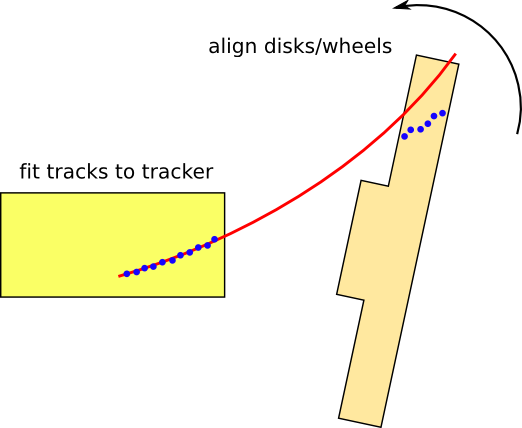
\includegraphics[width=0.4\linewidth]{globalMuon_alignment.png}

\vspace{-0.75 cm}
\hspace{-0.83 cm} \textcolor{darkblue}{\Large Reminder of method}

\vspace{0.25 cm}
\begin{itemize}
\item Treat 5 barrel wheels and 6 out of 8 endcap disks as 6-dof \mbox{rigid bodies\hspace{-1 cm}}
\item Select CRAFT global cosmic rays passing through tracker and wheel/disk
\item Fit tracker part, propagate to wheel/disk, align wheel/disk
\begin{itemize}
\item ME$\pm$4/1 and inner rings (ME$\pm$1/1, 2/1, 3/1) are nearly
  inaccessible (dozens of poor-quality tracks)
\item track-fitting and alignment step are independent
\end{itemize}
\item Every track residual can be converted into 6-dof \mbox{alignment corrections\hspace{-1 cm}}
\end{itemize}

\end{frame}

%% \section*{First section}
%% \begin{frame}
%% \begin{center}
%% \Huge \textcolor{blue}{First section}
%% \end{center}
%% \end{frame}


\begin{frame}
\frametitle{Selecting tracks by $p_T$}

\begin{columns}
\column{0.6\linewidth}

\begin{itemize}
\item CRAFT offers new ability to reject low-momentum tracks
\item Observe each alignment parameter as a function of curvature ($q/p_T$)
\item Cleanest measurement is \mbox{above 20~GeV\hspace{-1 cm}}
\end{itemize}

\begin{center}
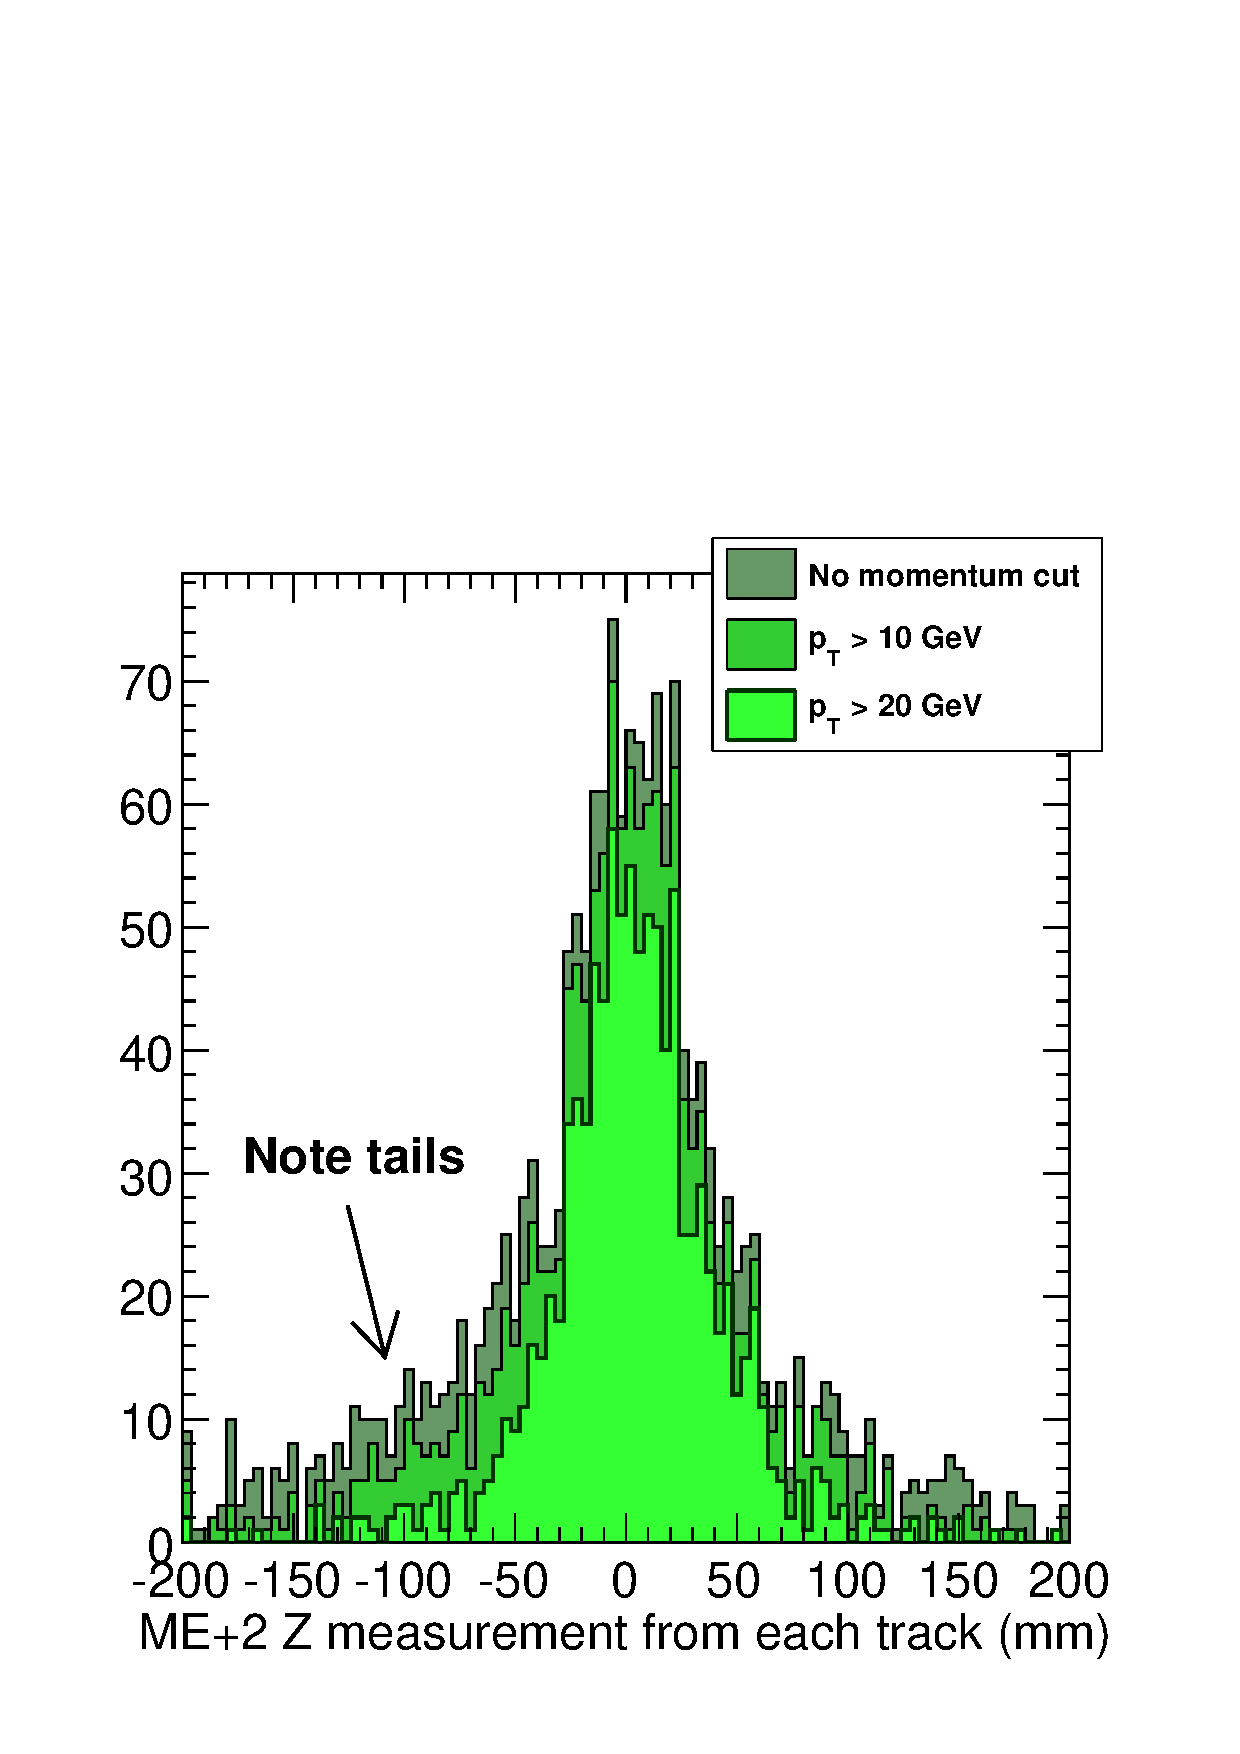
\includegraphics[width=0.75\linewidth]{measurement_from_each_track.pdf}
\end{center}

\column{0.4\linewidth}
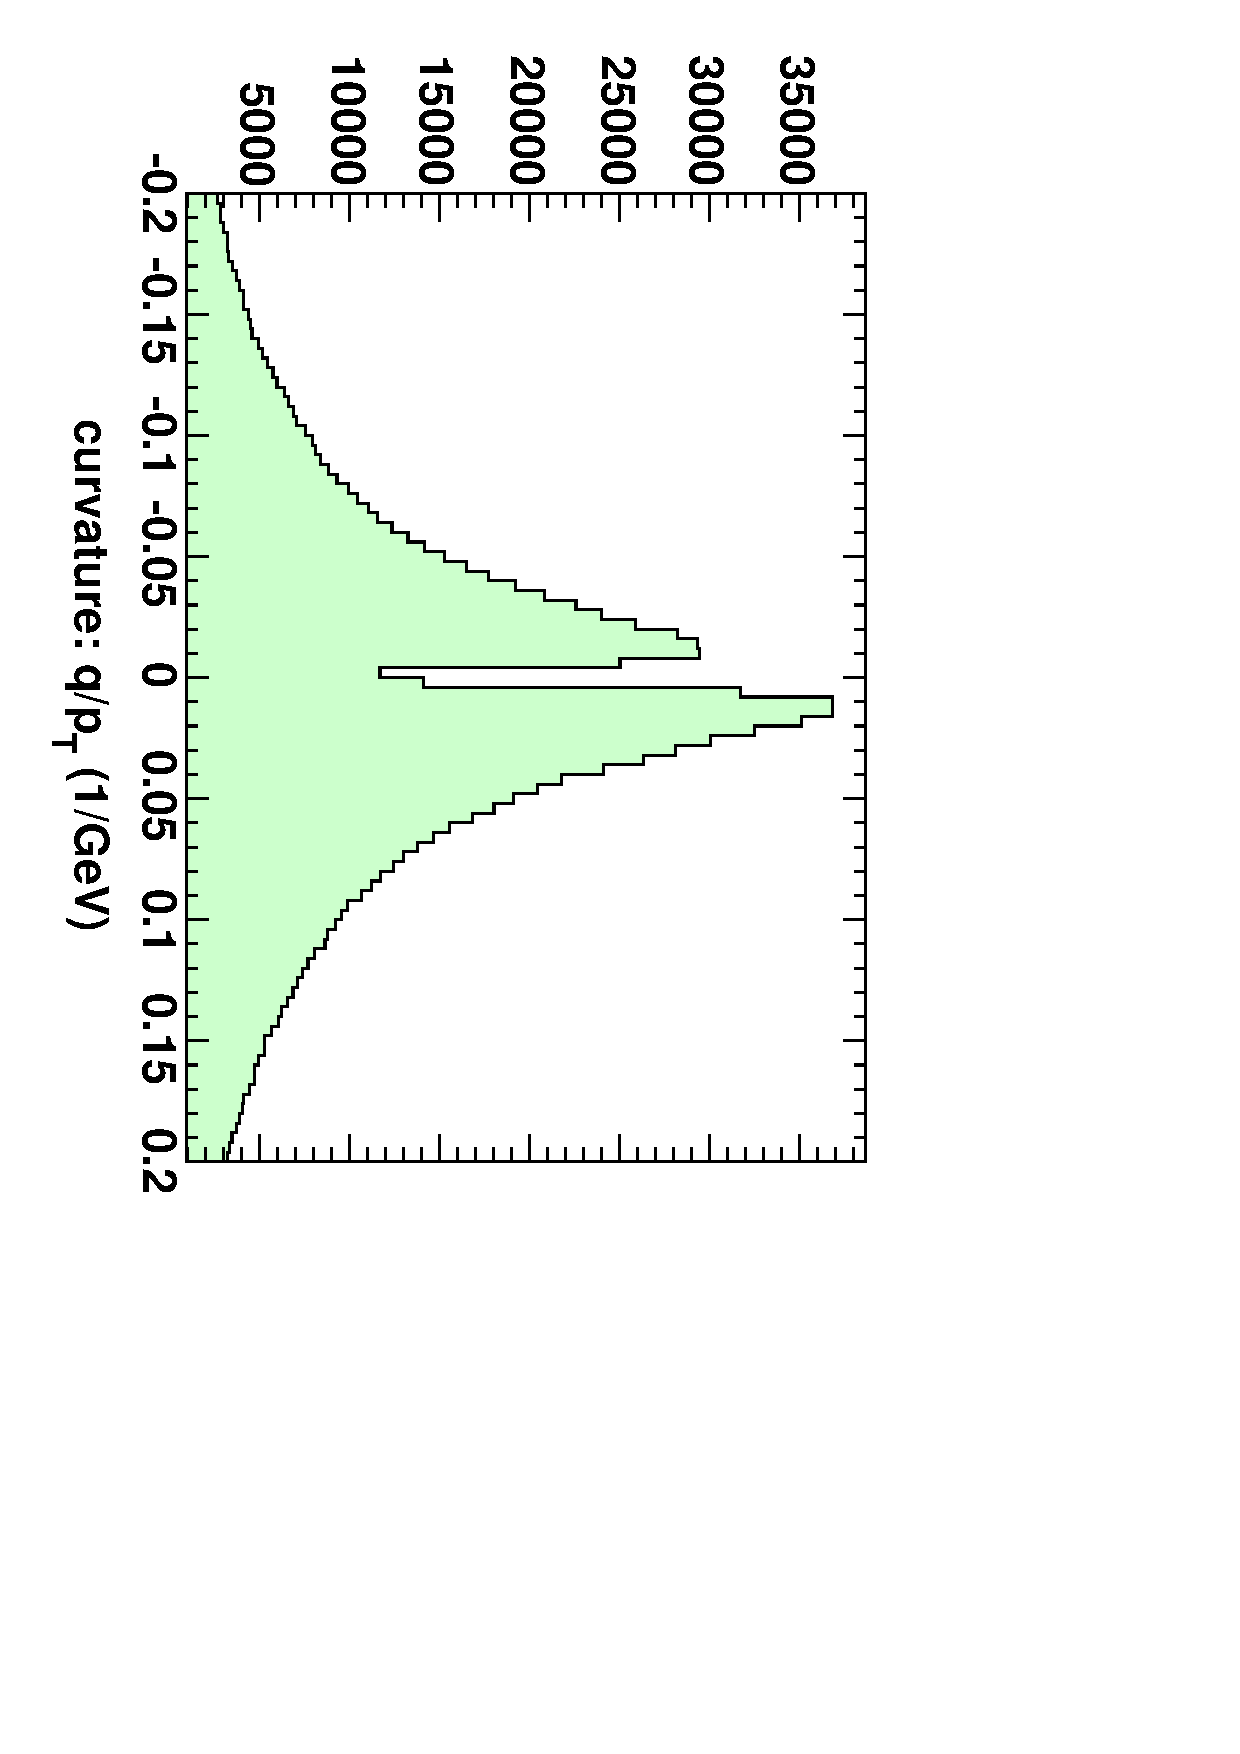
\includegraphics[height=\linewidth, angle=90]{qoverpt.pdf}

\vfill
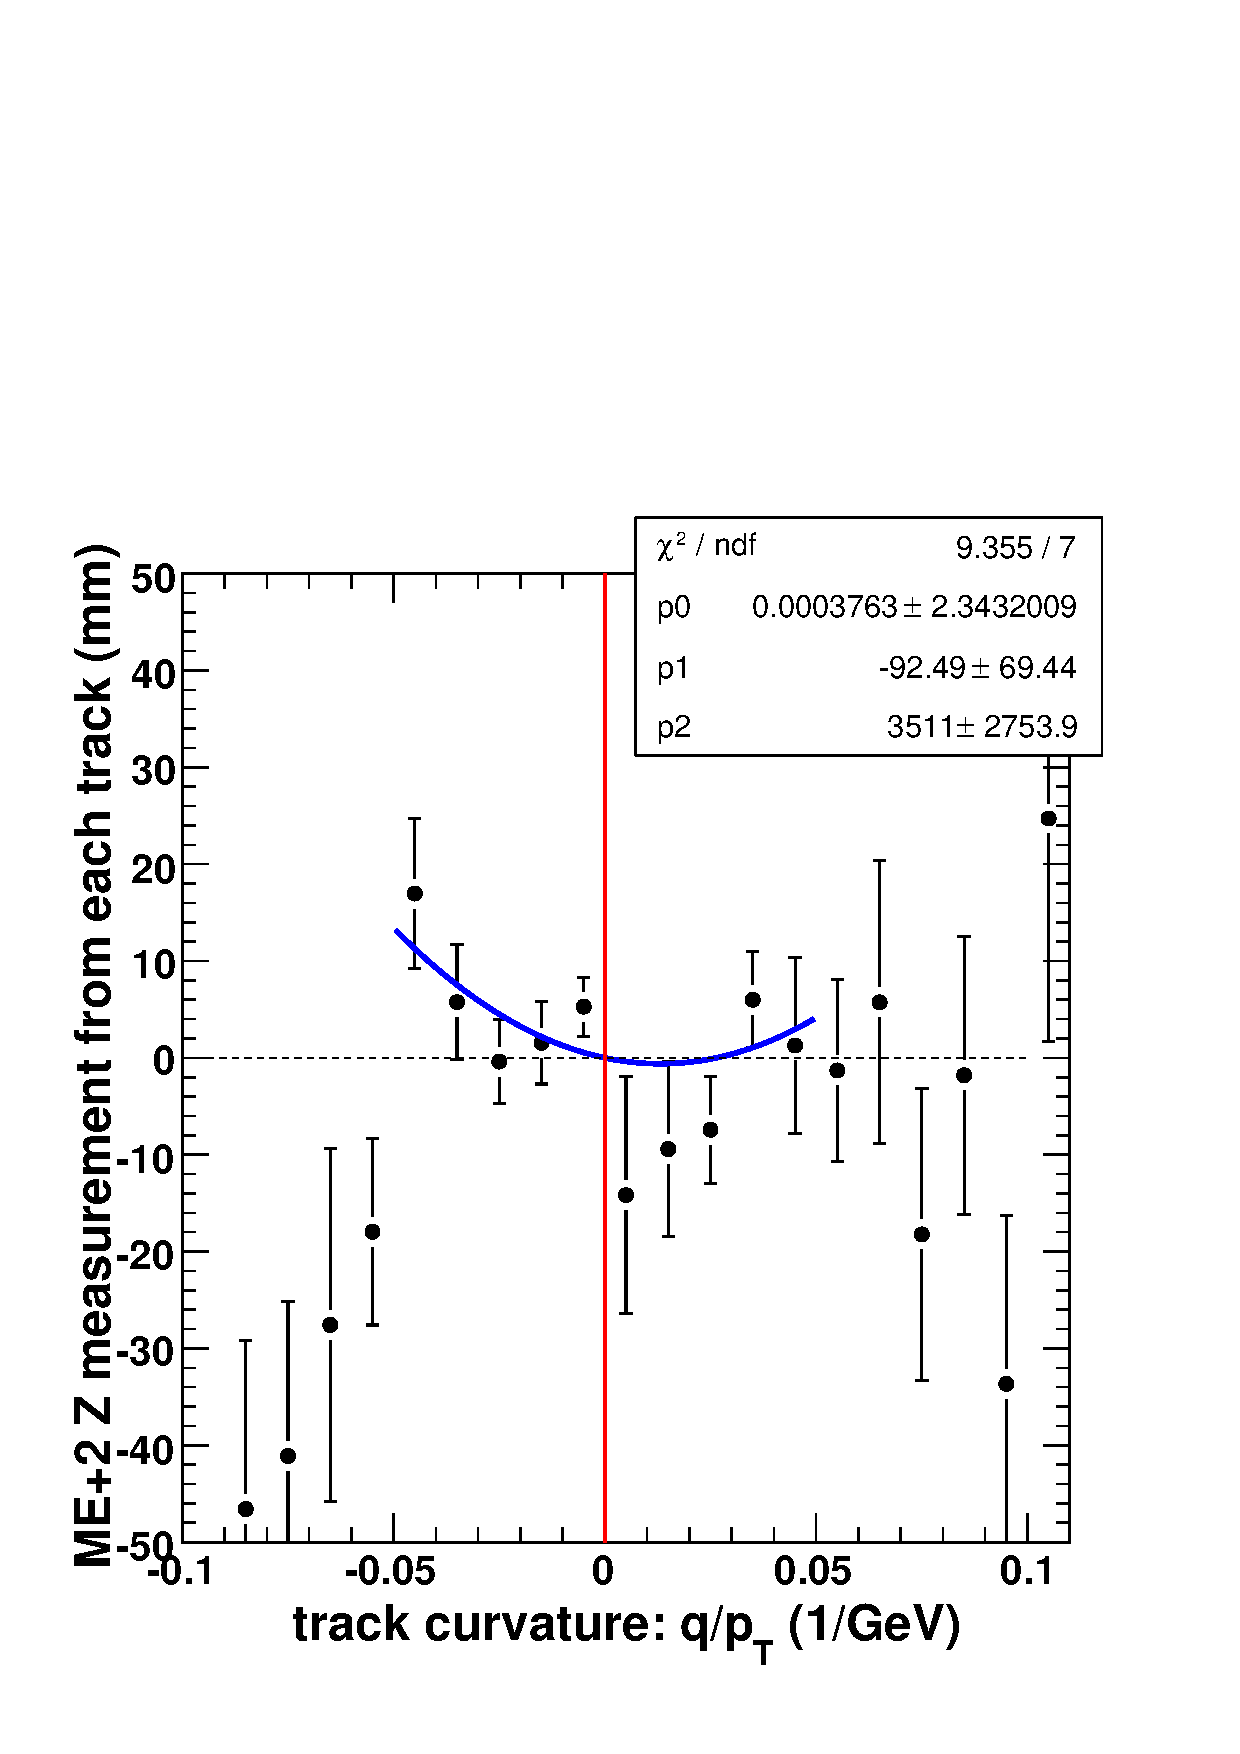
\includegraphics[width=\linewidth]{extrapolation_to_infinite_momentum.pdf}
\end{columns}
\end{frame}

\begin{frame}
\frametitle{$p \to \infty$ extrapolation}

\begin{itemize}
\item Multiple scattering and $\vec{B}$ errors limit to zero at infinite momentum
\begin{itemize}
\item multiple scattering is symmetric (independent of $q$)
\item $\vec{B}$ errors are antisymmetric with $q$
\item both depend on track angles and detailed track distribution
\end{itemize}

\item Taylor-expand around $q/p_T = 0$ up to second order
\item \textcolor{darkblue}{Constant term ($p_0$) is the misalignment: alignment minimizes $p_0$}
\item Linear term ($p_1$) is $\vec{B}$ error, sensitive to a few percent of a Tesla
\end{itemize}

\begin{columns}
\column{0.33\linewidth}
\mbox{ } \hfill ME$+$2 $z$ \hfill \mbox{ }

\vspace{0.1 cm}
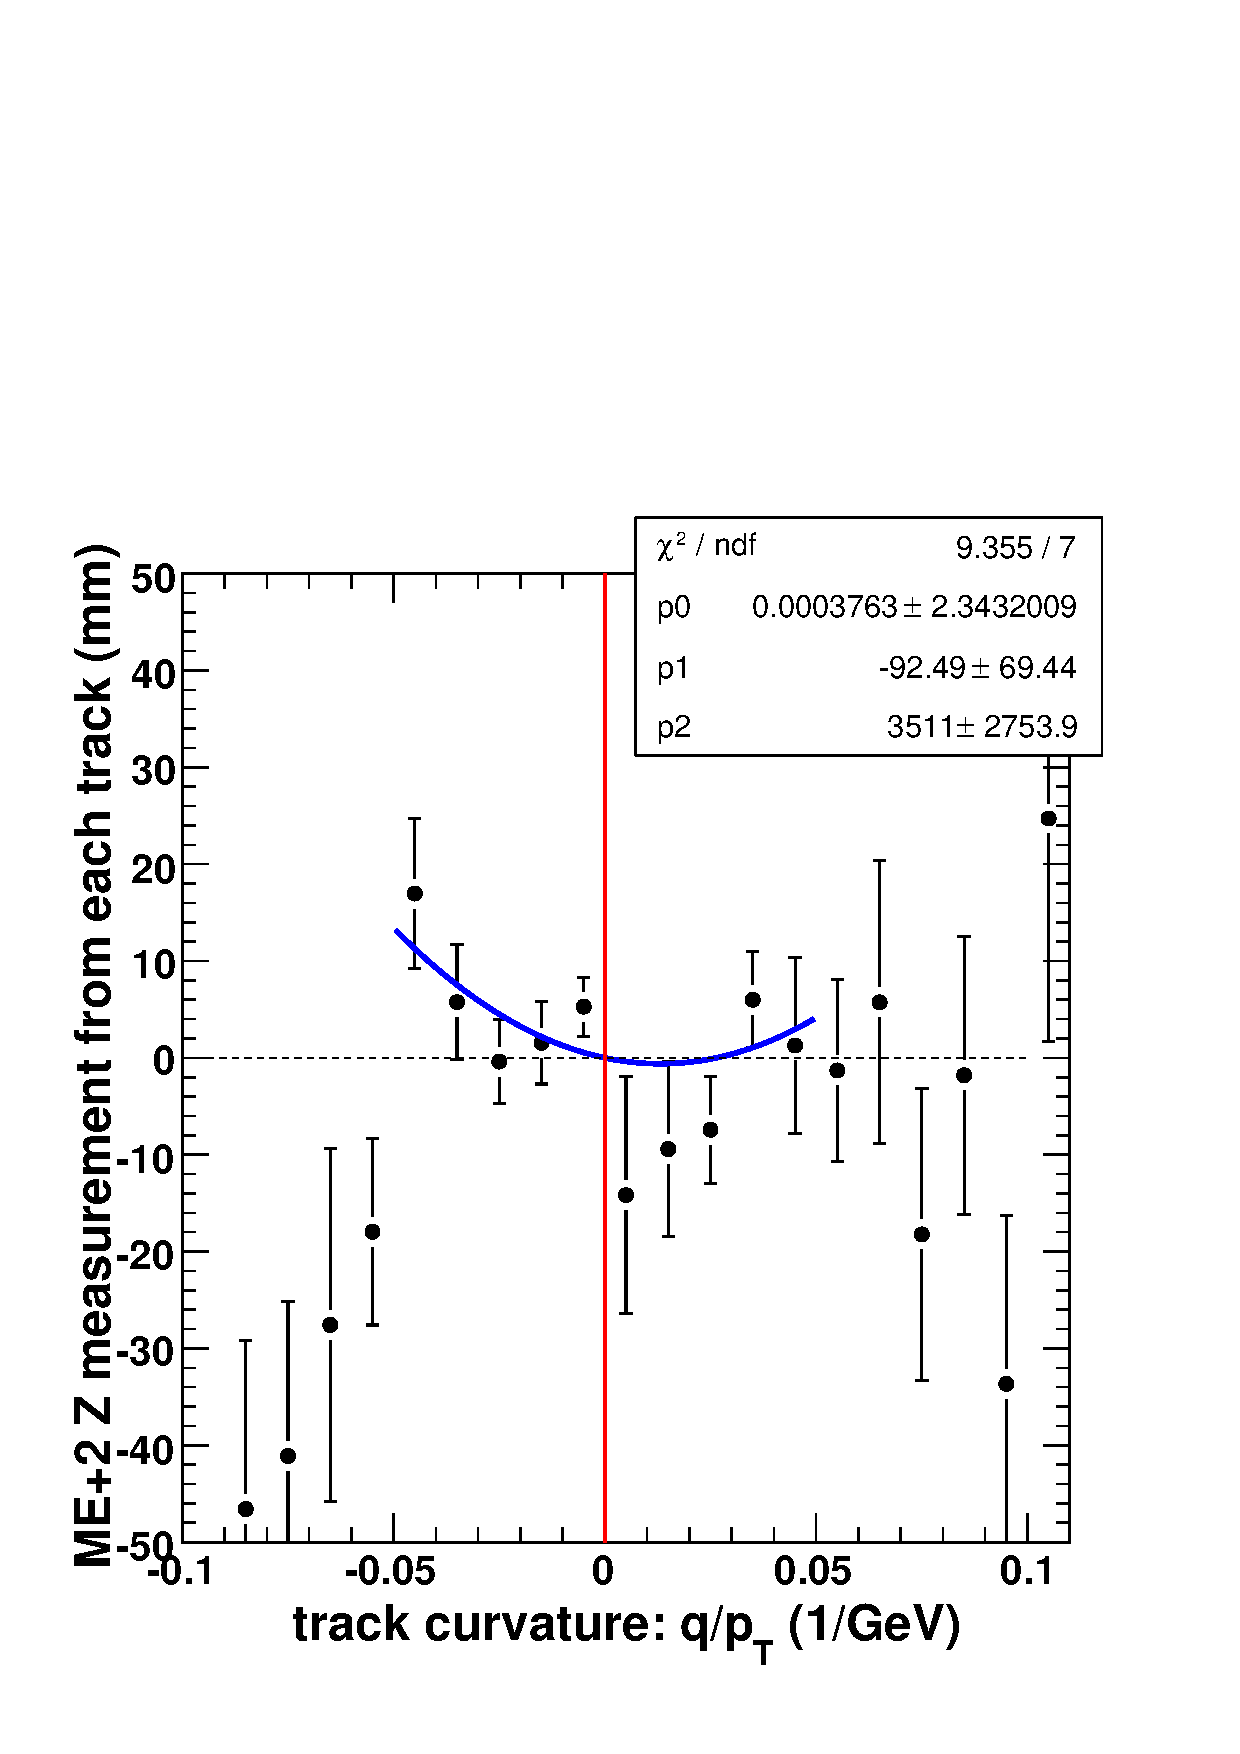
\includegraphics[width=\linewidth]{extrapolation_to_infinite_momentum.pdf}
\column{0.33\linewidth}
\mbox{ } \hfill Wheel 0 $z$ \hfill \mbox{ }

\vspace{0.1 cm}
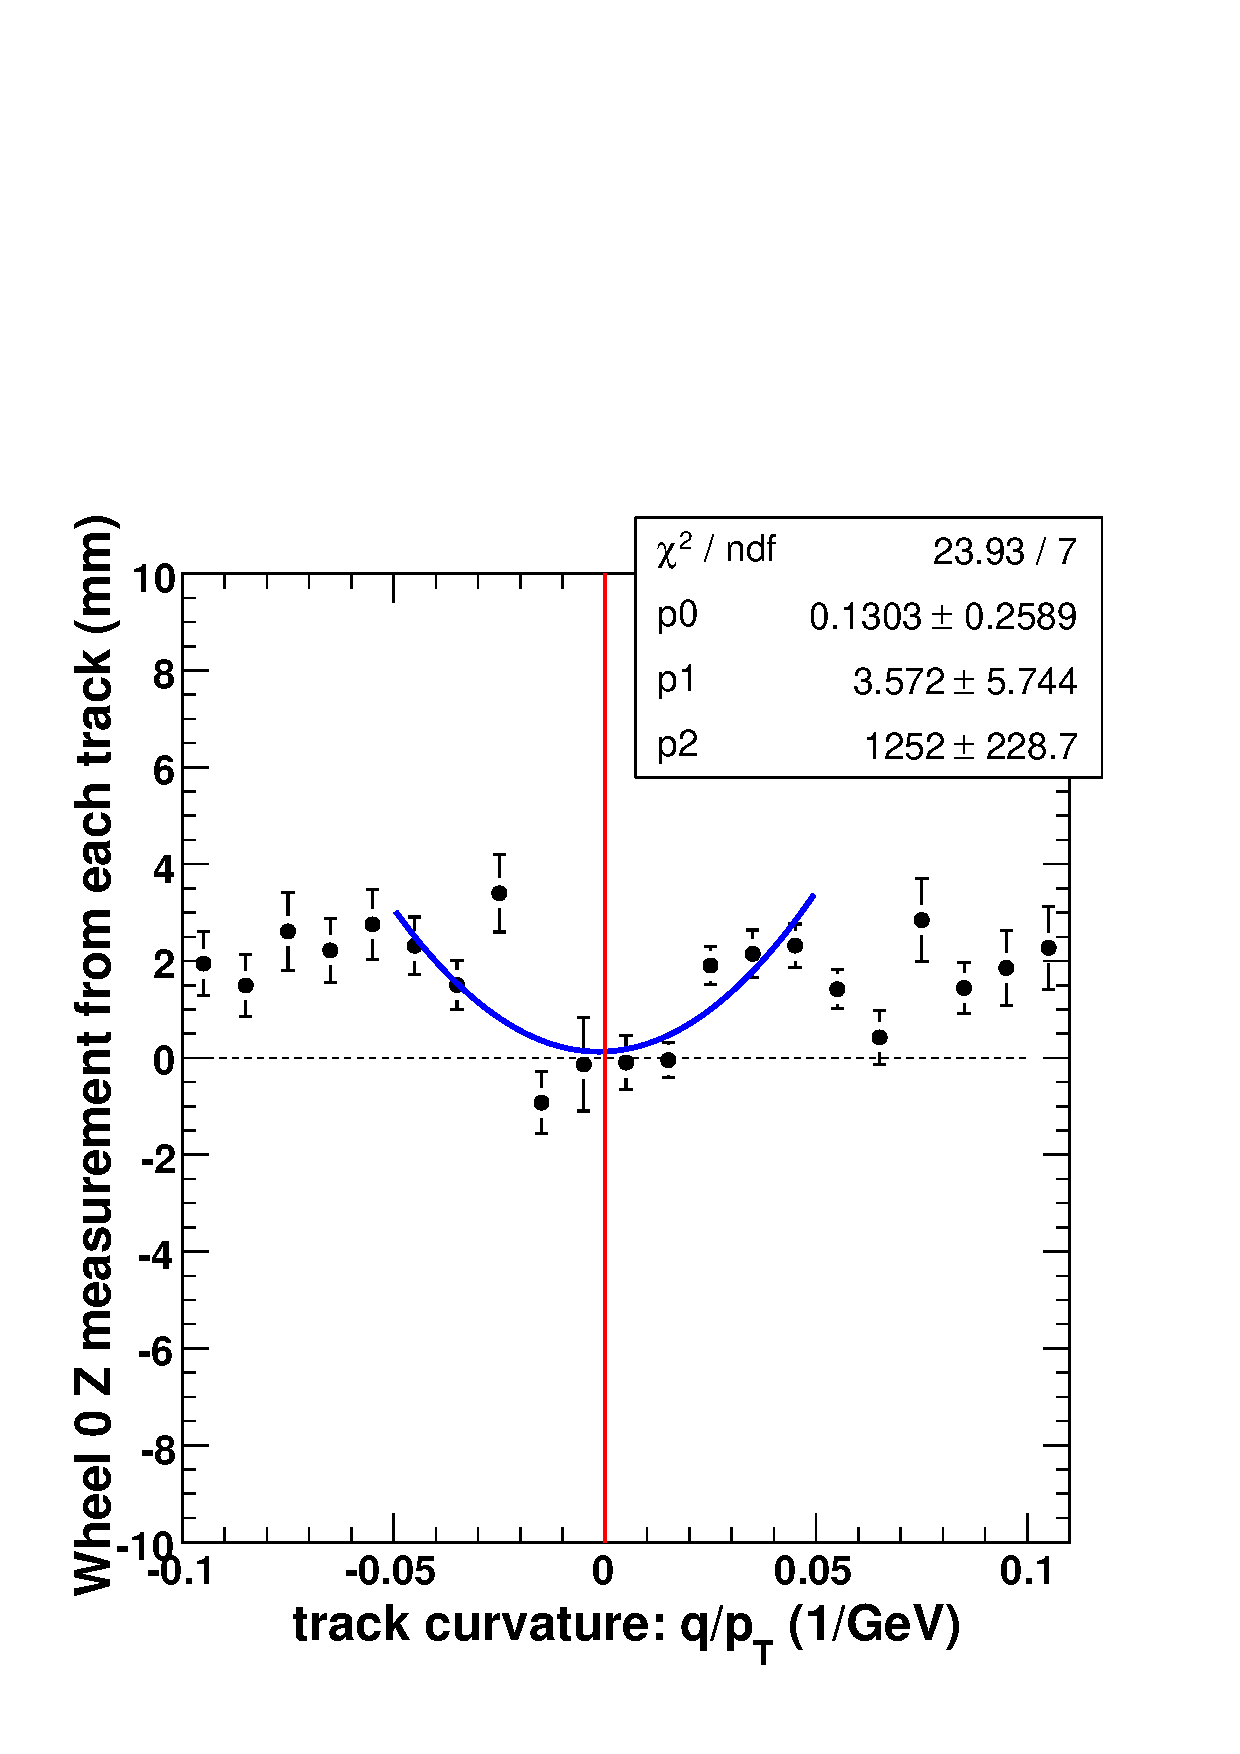
\includegraphics[width=\linewidth]{extrapolation_wheel0.pdf}
\column{0.33\linewidth}
\mbox{ } \hfill ME$+$2 $\phi_z$ \hfill \mbox{ }

\vspace{0.1 cm}
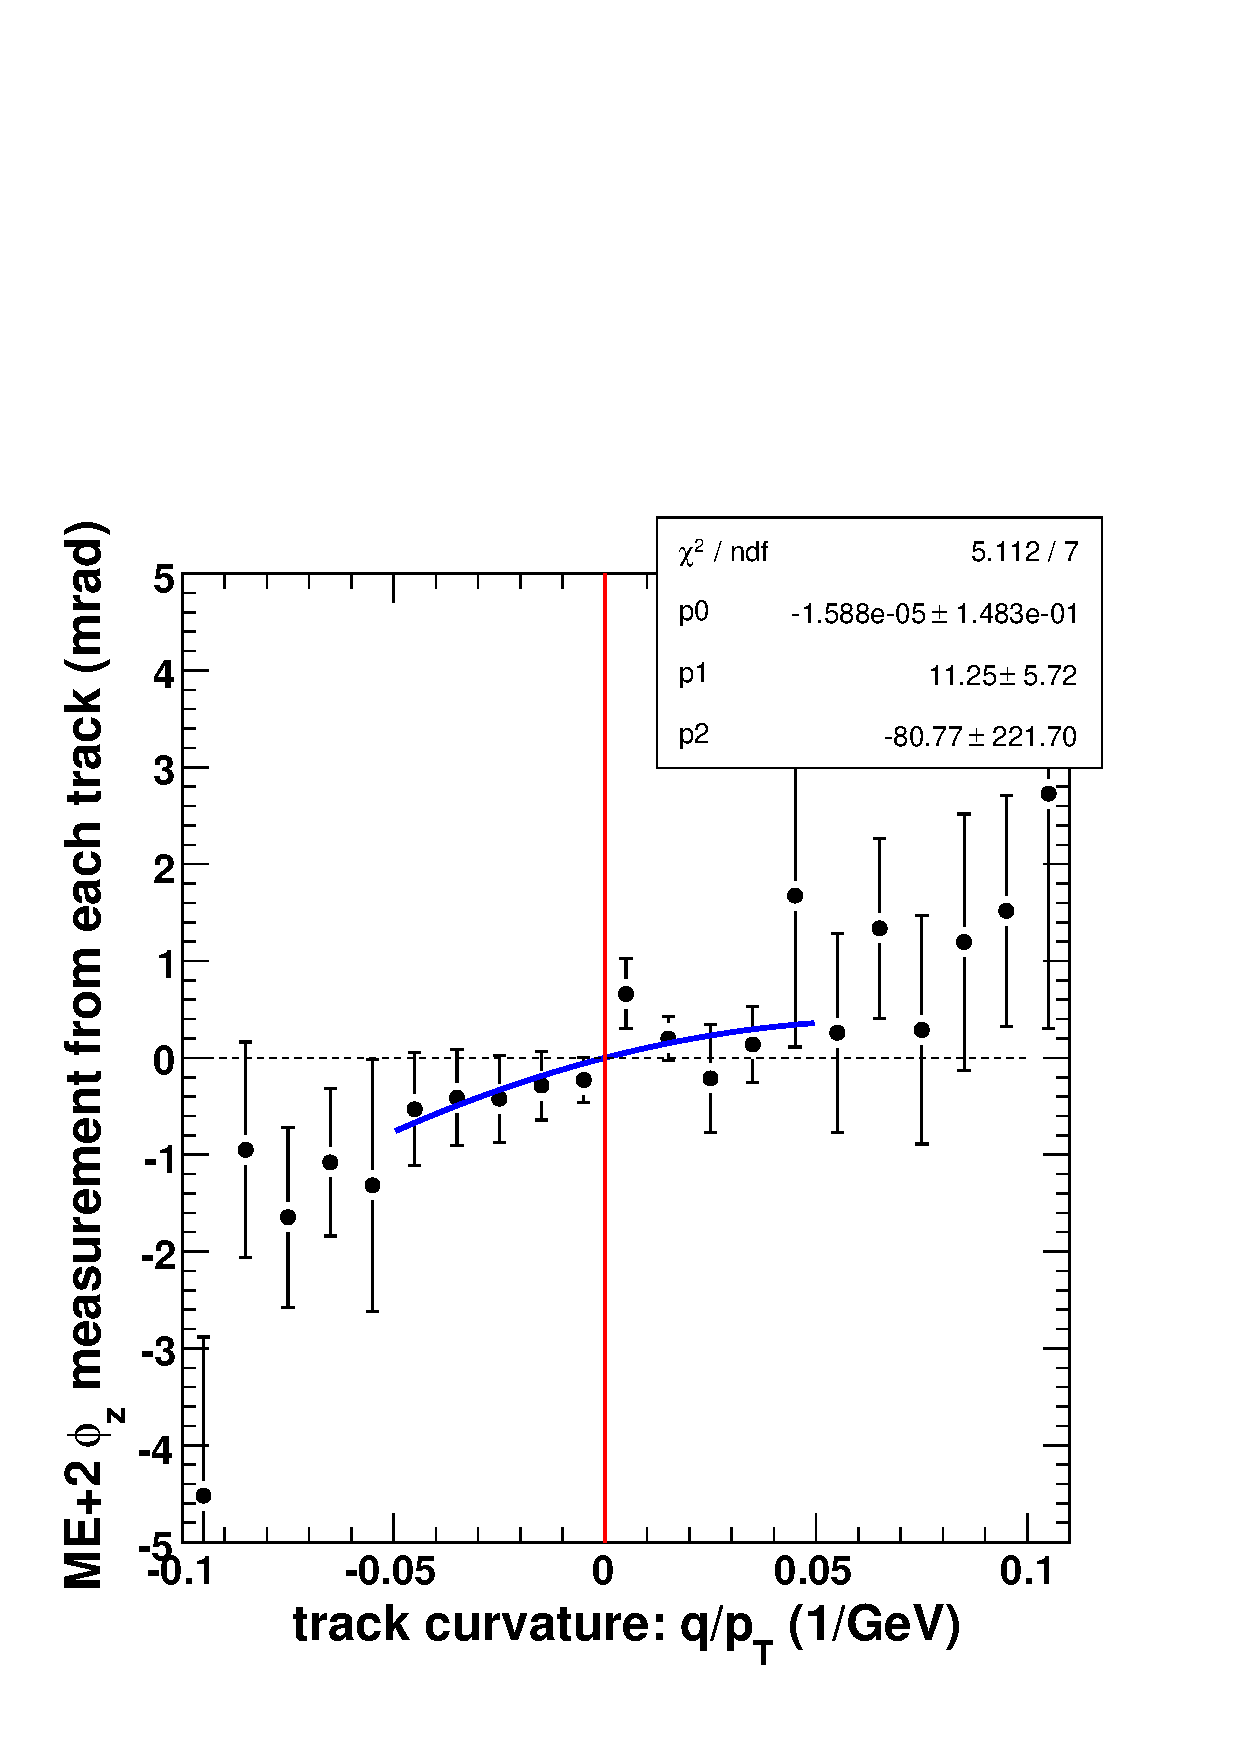
\includegraphics[width=\linewidth]{extrapolation_phiz.pdf}
\end{columns}
\end{frame}

\begin{frame}
\frametitle{Details}
\begin{itemize}\setlength{\itemsep}{0.1 cm}
\item Iteration scheme: $2\times \left(\begin{array}{c} z \\ \phi_z \end{array}\right)$, followed by
$4\times \left(\begin{array}{c c c} x & y & z \\ \phi_x & \phi_y & \phi_z \end{array}\right)$
\begin{itemize}
\item only needed for resolving correlations among parameters: track-fits
  are already independent of muon alignment
\end{itemize}

\item All barrel wheels converged, endcap disks only in $\left(\begin{array}{c} z \\ \phi_z \end{array}\right)$ scheme
\begin{itemize}
\item I think I only need to fix $y$ for endcap (converged in early tests)
\end{itemize}

\item Endcap disks aligned with tracks passing through outer ring only
  (allows inner ring correction to be applied from \mbox{hardware measurement)\hspace{-1 cm}}

\item Barrel wheels: weighted means \\
Endcap disks: unweighted means (due to low statistics)
\begin{itemize}
\item Barrel uncertainties are underestimated: switch back to unweighted means in future
\end{itemize}

\item Quality cuts: tracker $\chi^2/N_{\mbox{\scriptsize DOF}} < 10$,
  $N_{\mbox{\scriptsize tracker hits}} \ge 10$, at least 500 tracks
  per alignable

\item I check quality of each ``parameter vs.\ $q/p_T$'' fit manually

\end{itemize}
\end{frame}

\begin{frame}
\frametitle{All alignment results (\only<1>{1}\only<2>{2}\only<3>{3}\only<4>{4}\only<5>{5}\only<6>{6}\only<7>{7}\only<8>{8}/8)}

\vfill
\begin{itemize}
\item Four run regions with stable 3.8~T field
\item Results depend on tracker alignment: this uses \only<1,3,5,7>{tracker-HIP}\only<2,4,6,8>{tracker-MillePede}\uncover<1,3,5,7>{ with survey constraints}
\item Muon alignment uses tracks only \only<1,2>{(aligned is {\it contracted} \mbox{relative to ideal)\hspace{-1 cm}}}\only<3,4>{(\textcolor{purple}{$\Delta$} has smallest $N_{\mbox{\scriptsize tracks}}$)}
\item From the pattern, I do not believe run-by-run differences are real
\end{itemize}

\vfill
\only<1>{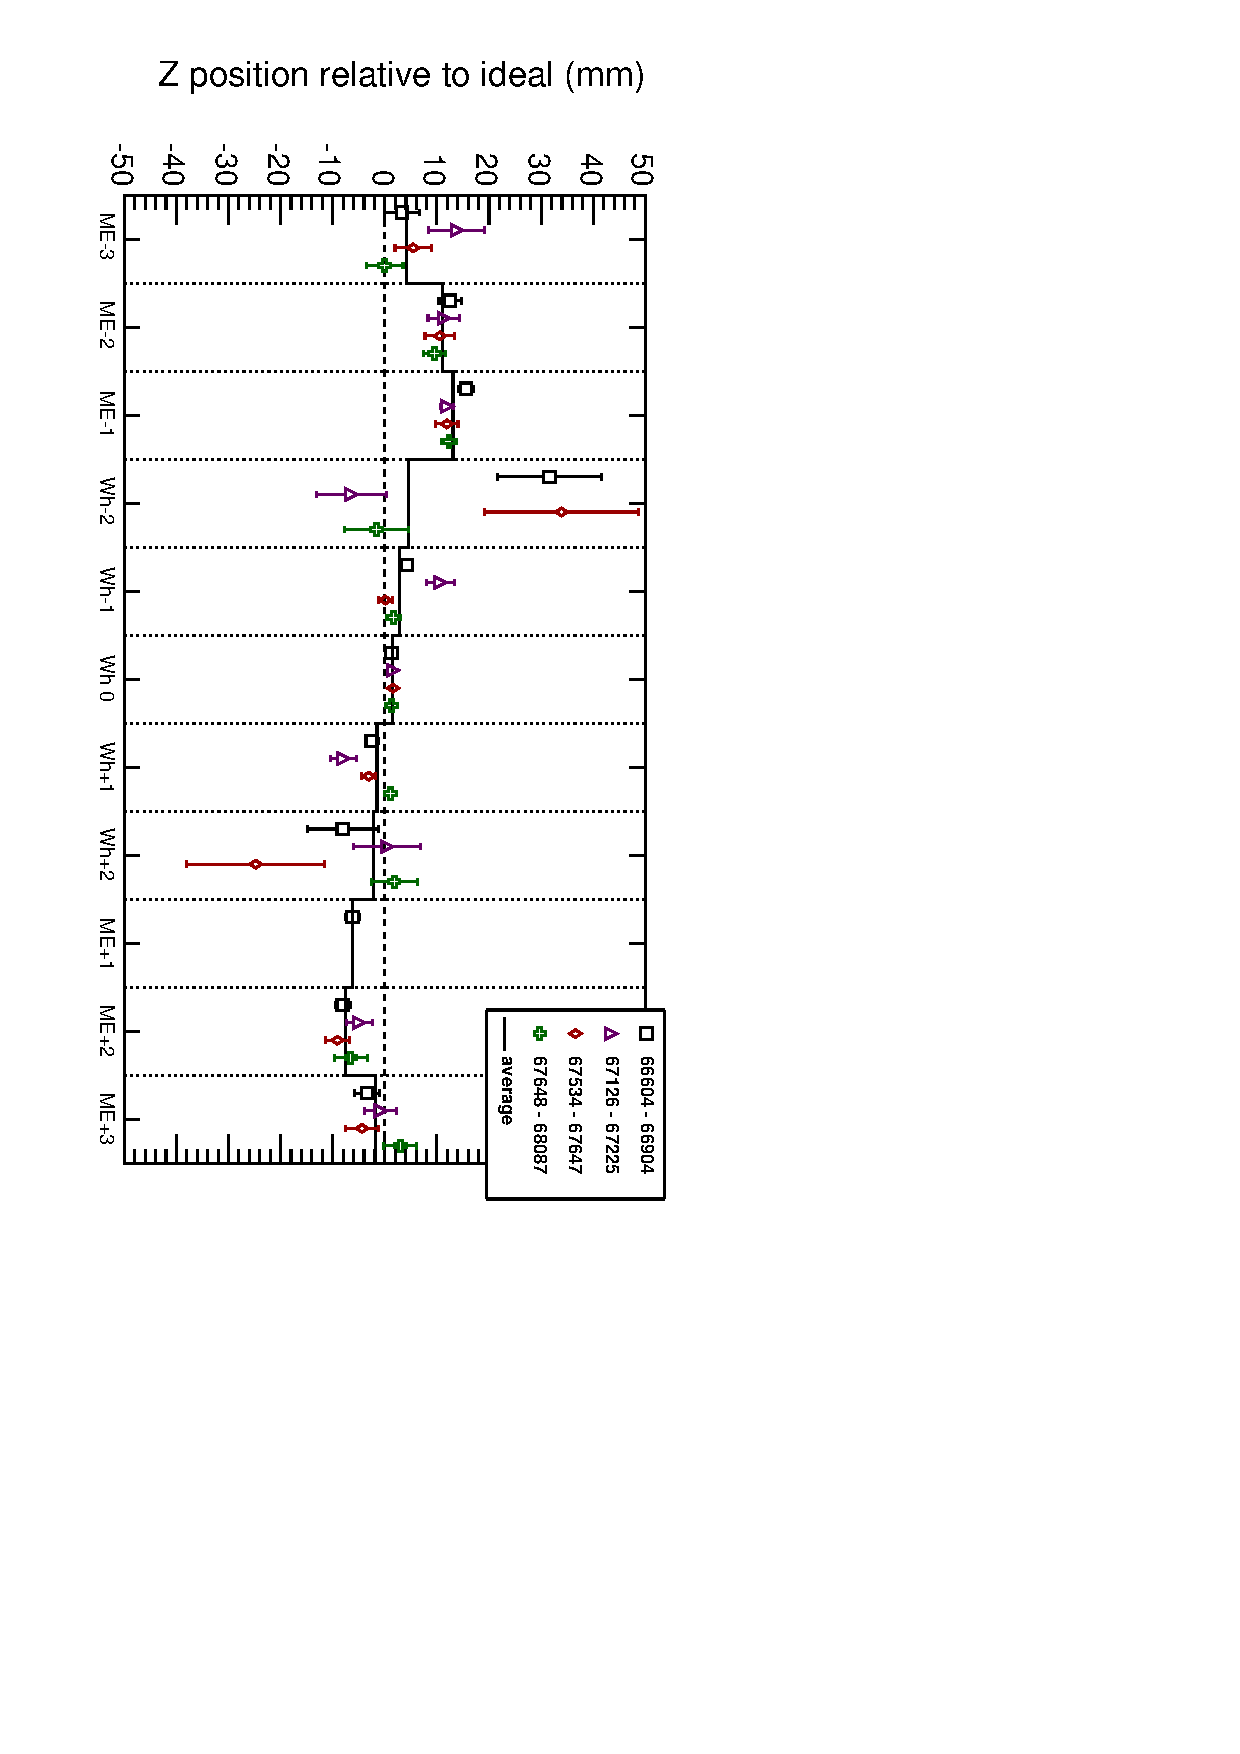
\includegraphics[height=\linewidth, angle=90]{bydataset_HIPSC_z.pdf}}
\only<2>{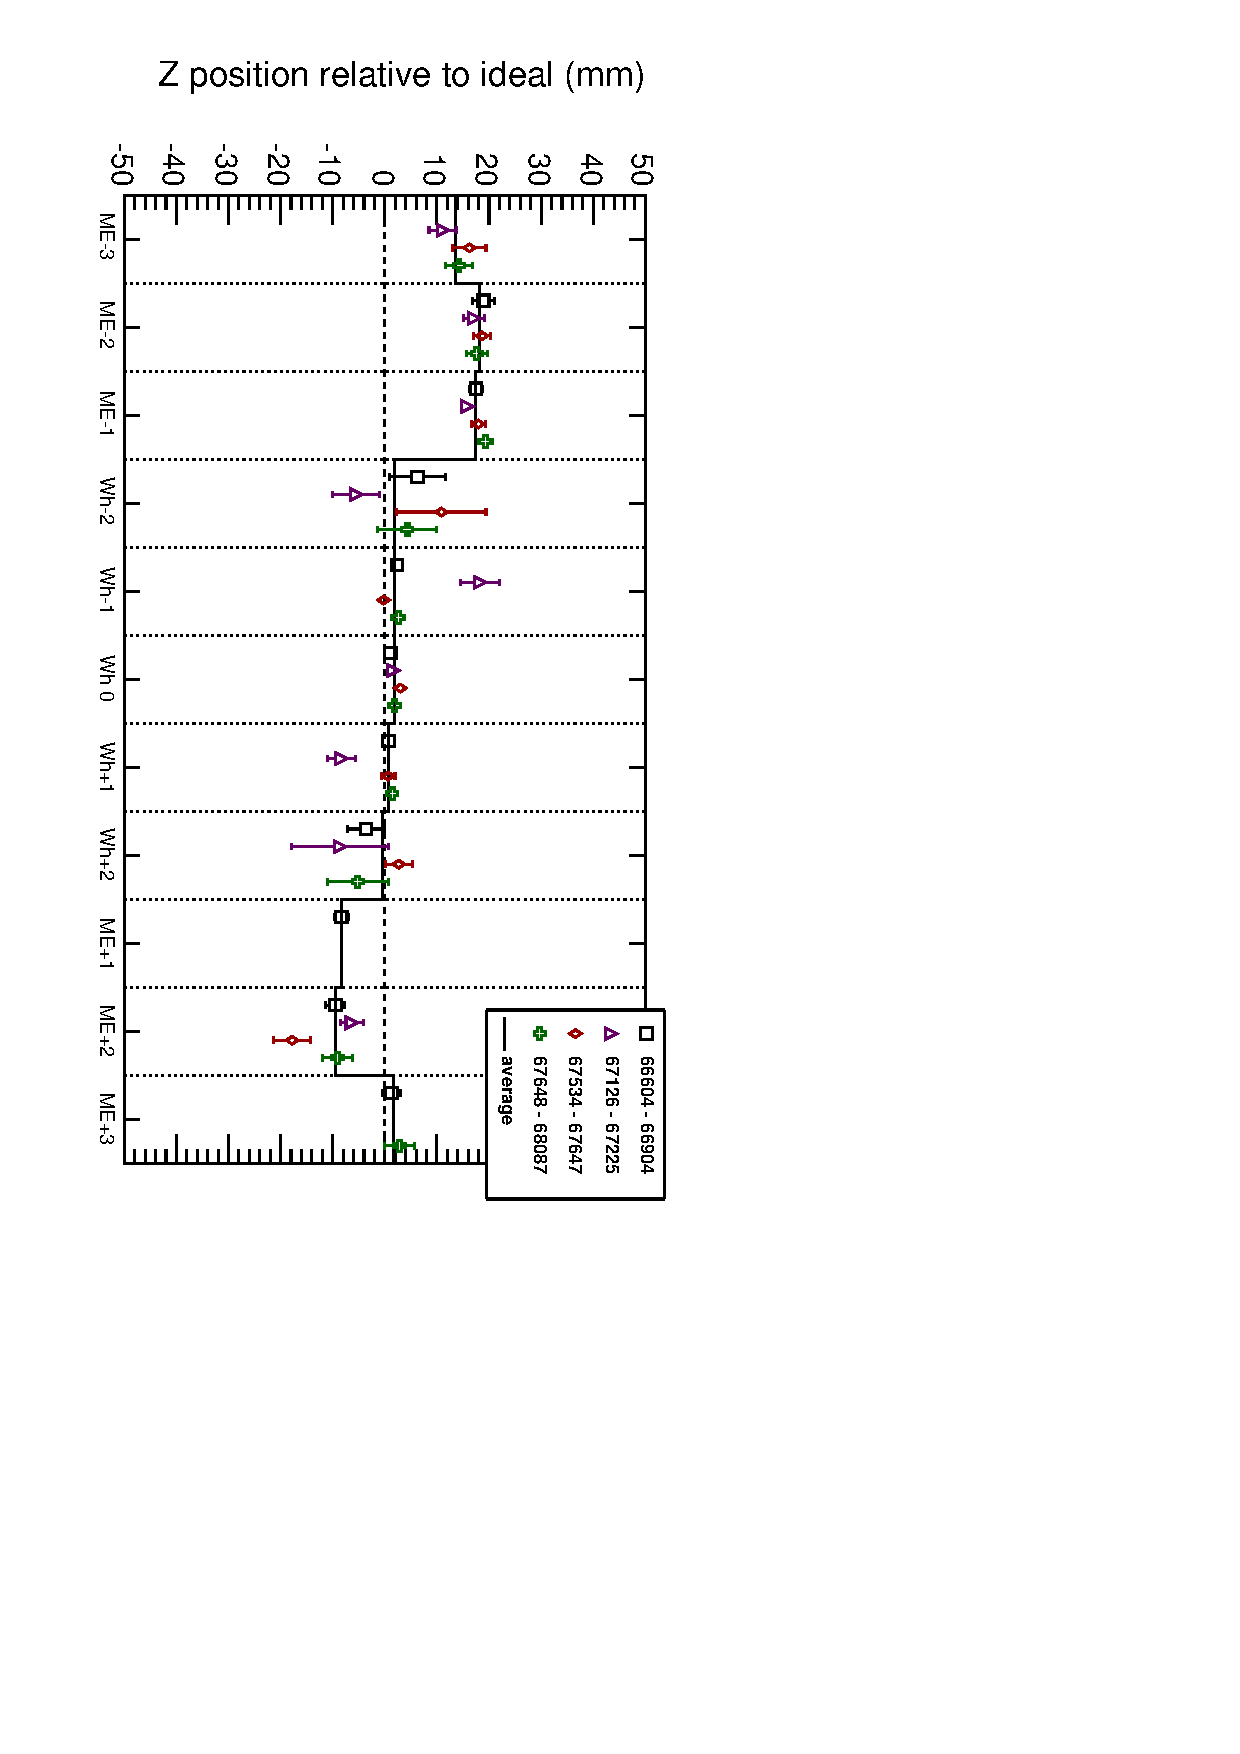
\includegraphics[height=\linewidth, angle=90]{bydataset_MP_z.pdf}}
\only<3>{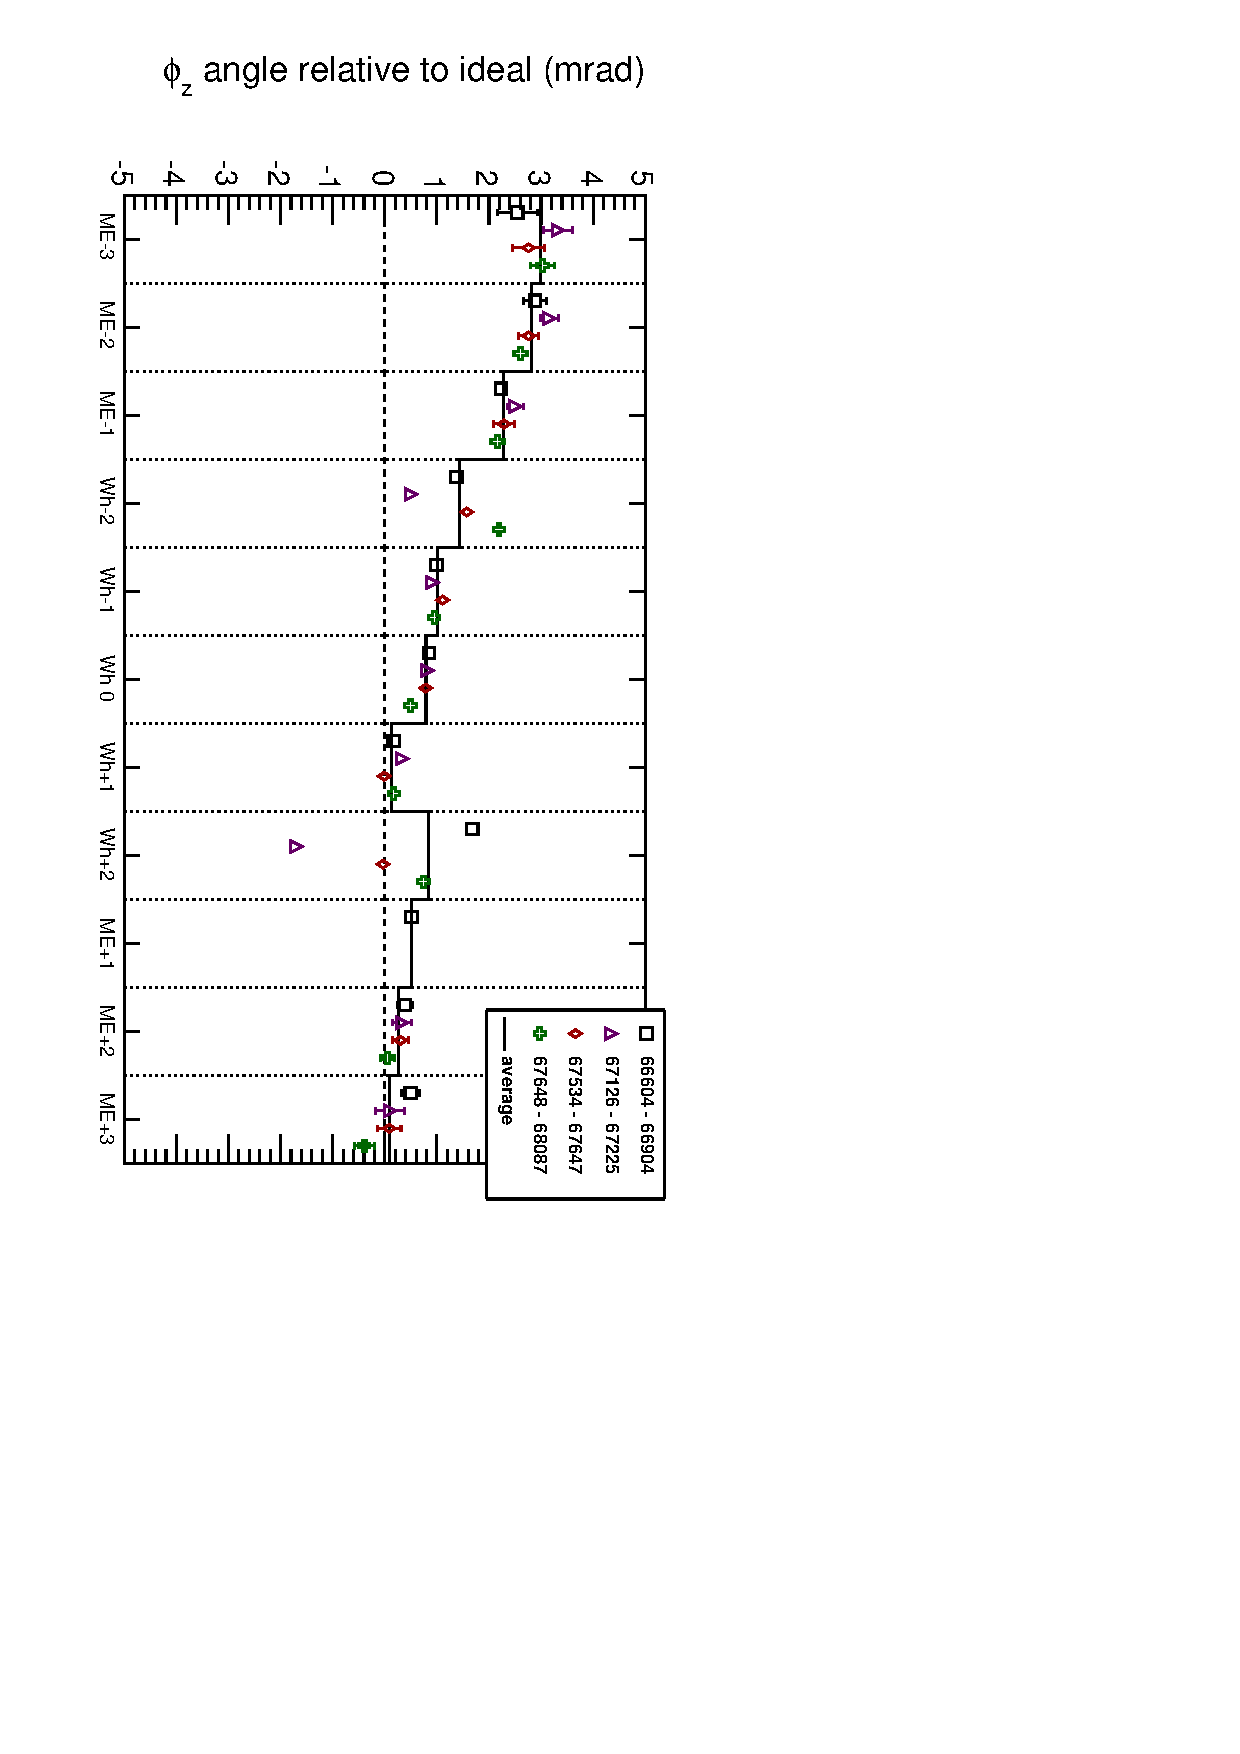
\includegraphics[height=\linewidth, angle=90]{bydataset_HIPSC_phiz.pdf}}
\only<4>{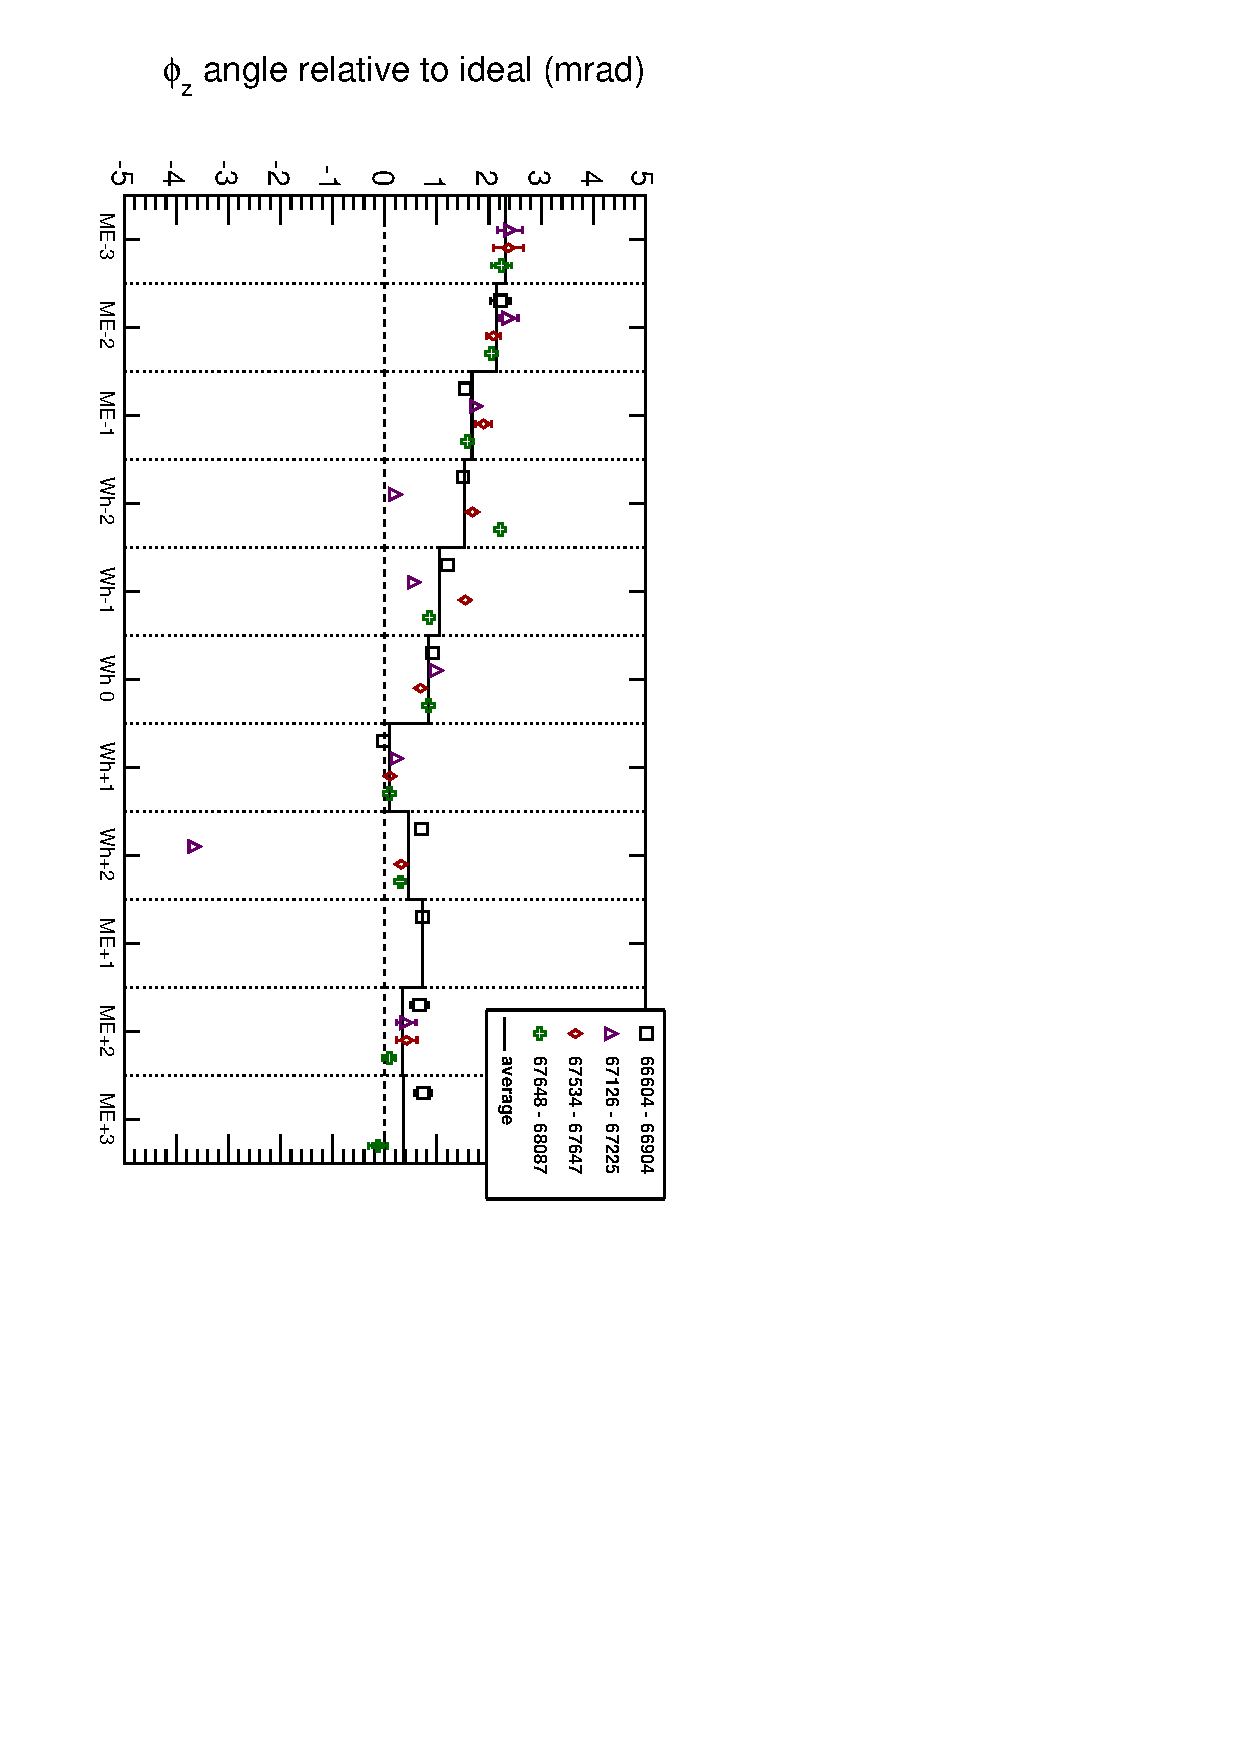
\includegraphics[height=\linewidth, angle=90]{bydataset_MP_phiz.pdf}}
\only<5>{\begin{columns}
\column{0.5\linewidth}
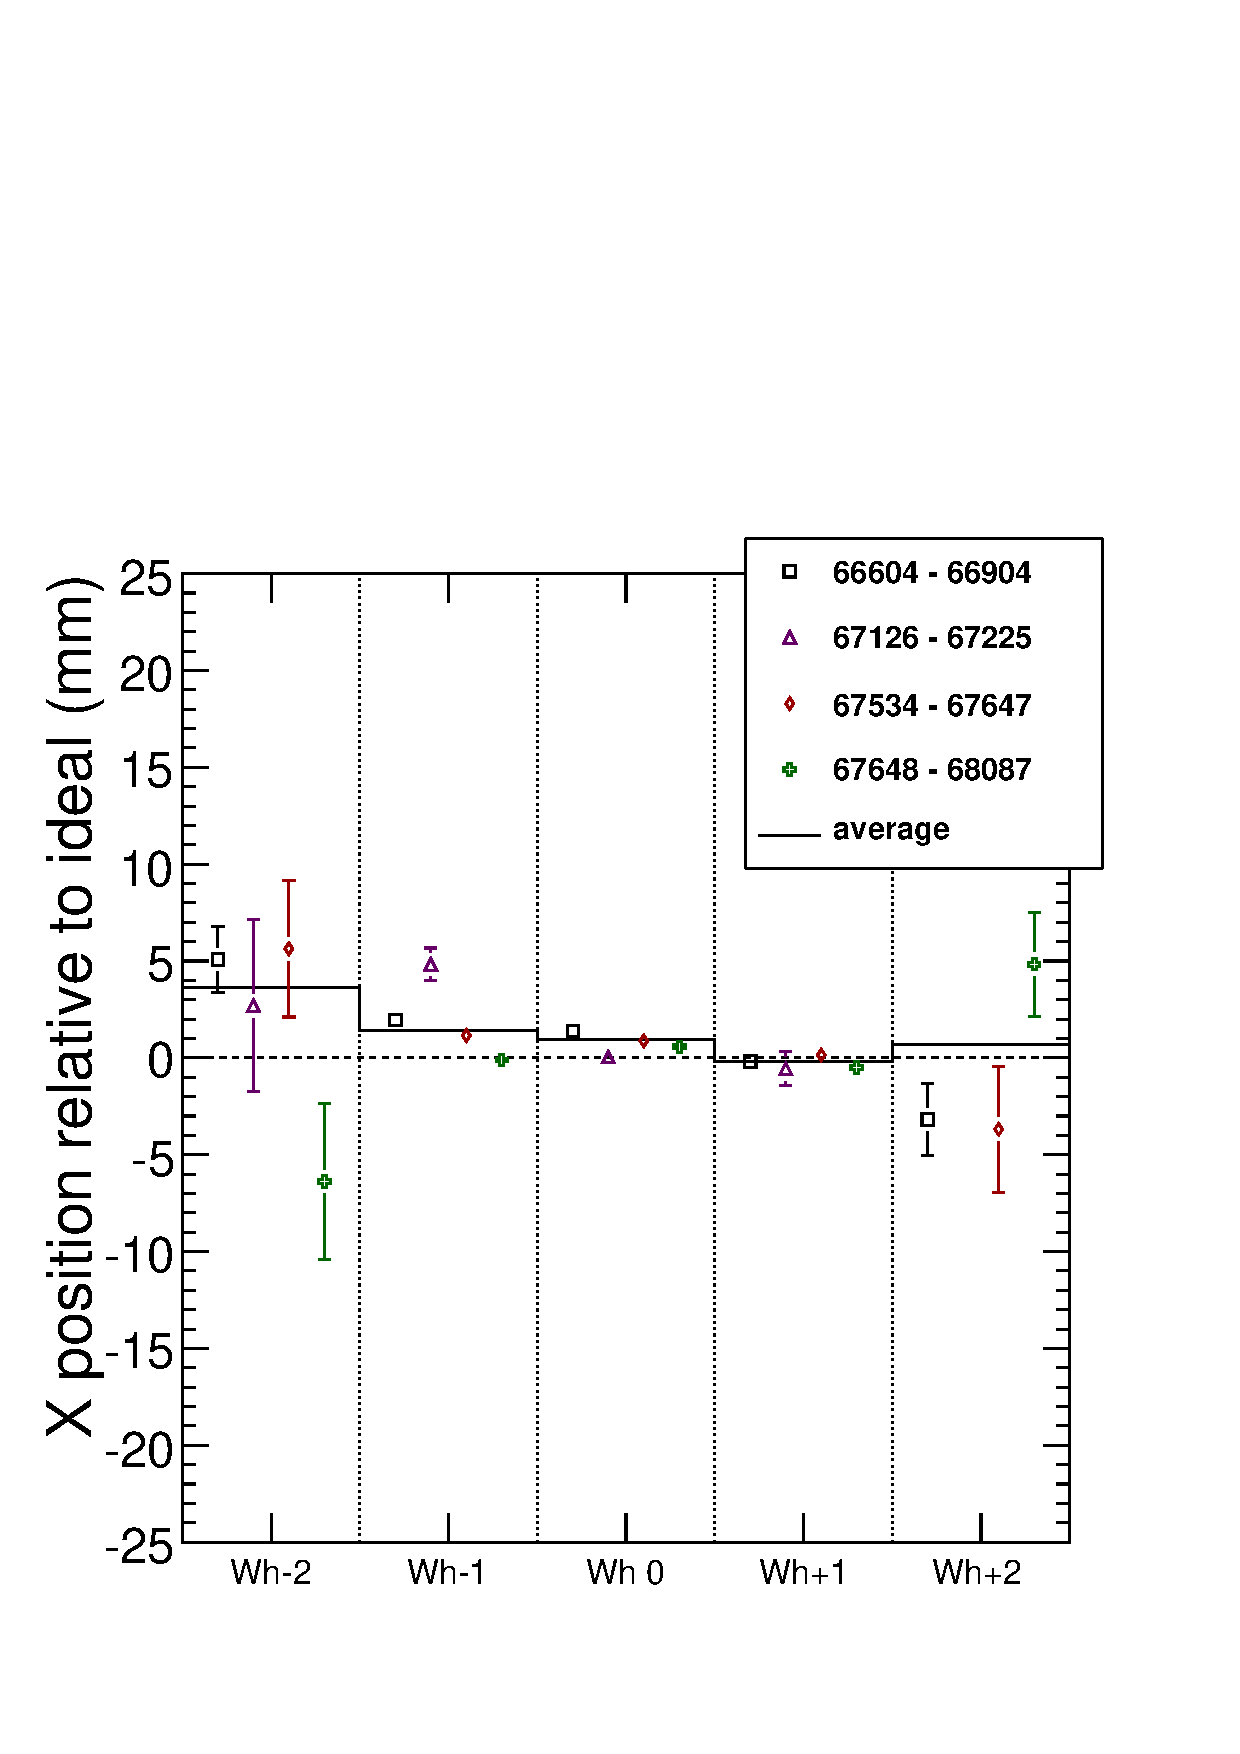
\includegraphics[width=\linewidth]{bydataset_HIPSC_x.pdf}
\column{0.5\linewidth}
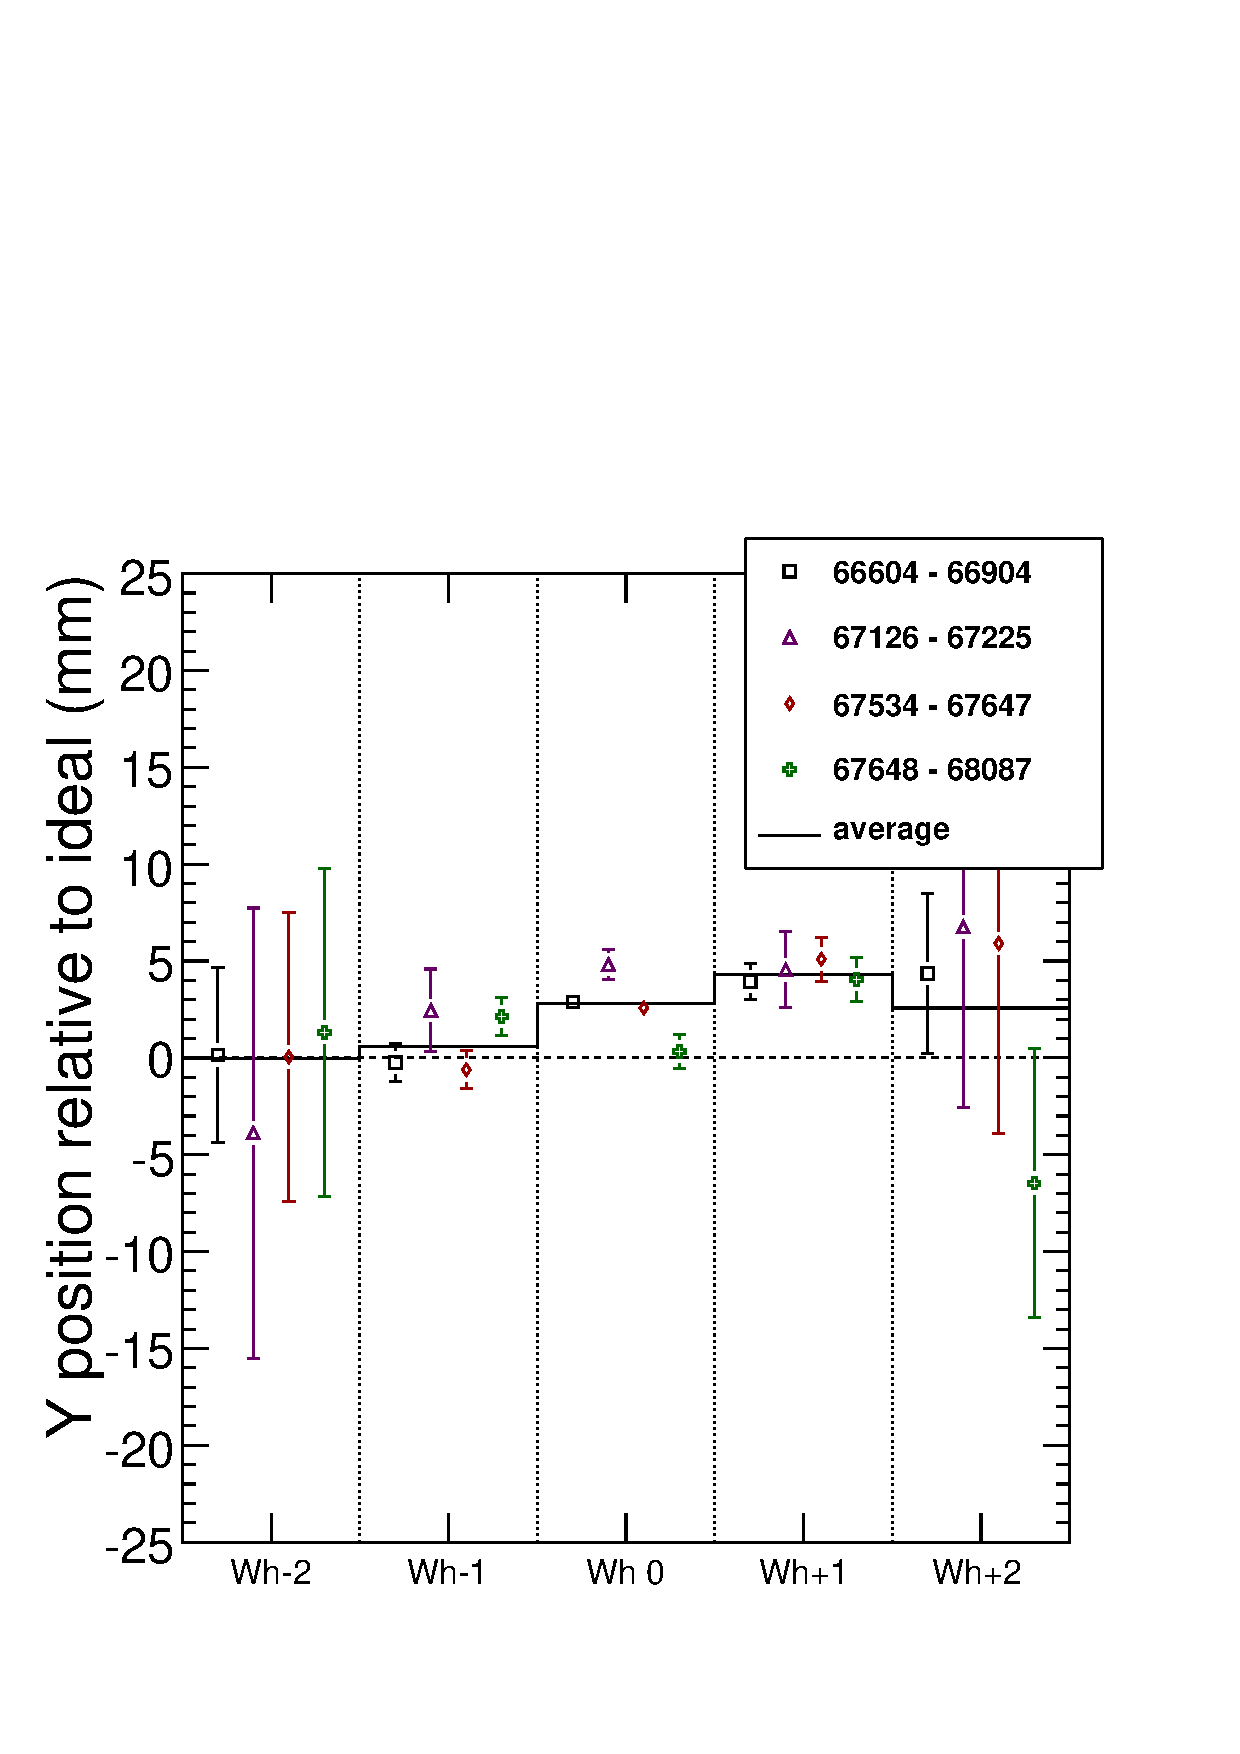
\includegraphics[width=\linewidth]{bydataset_HIPSC_y.pdf}
\end{columns}}
\only<6>{\begin{columns}
\column{0.5\linewidth}
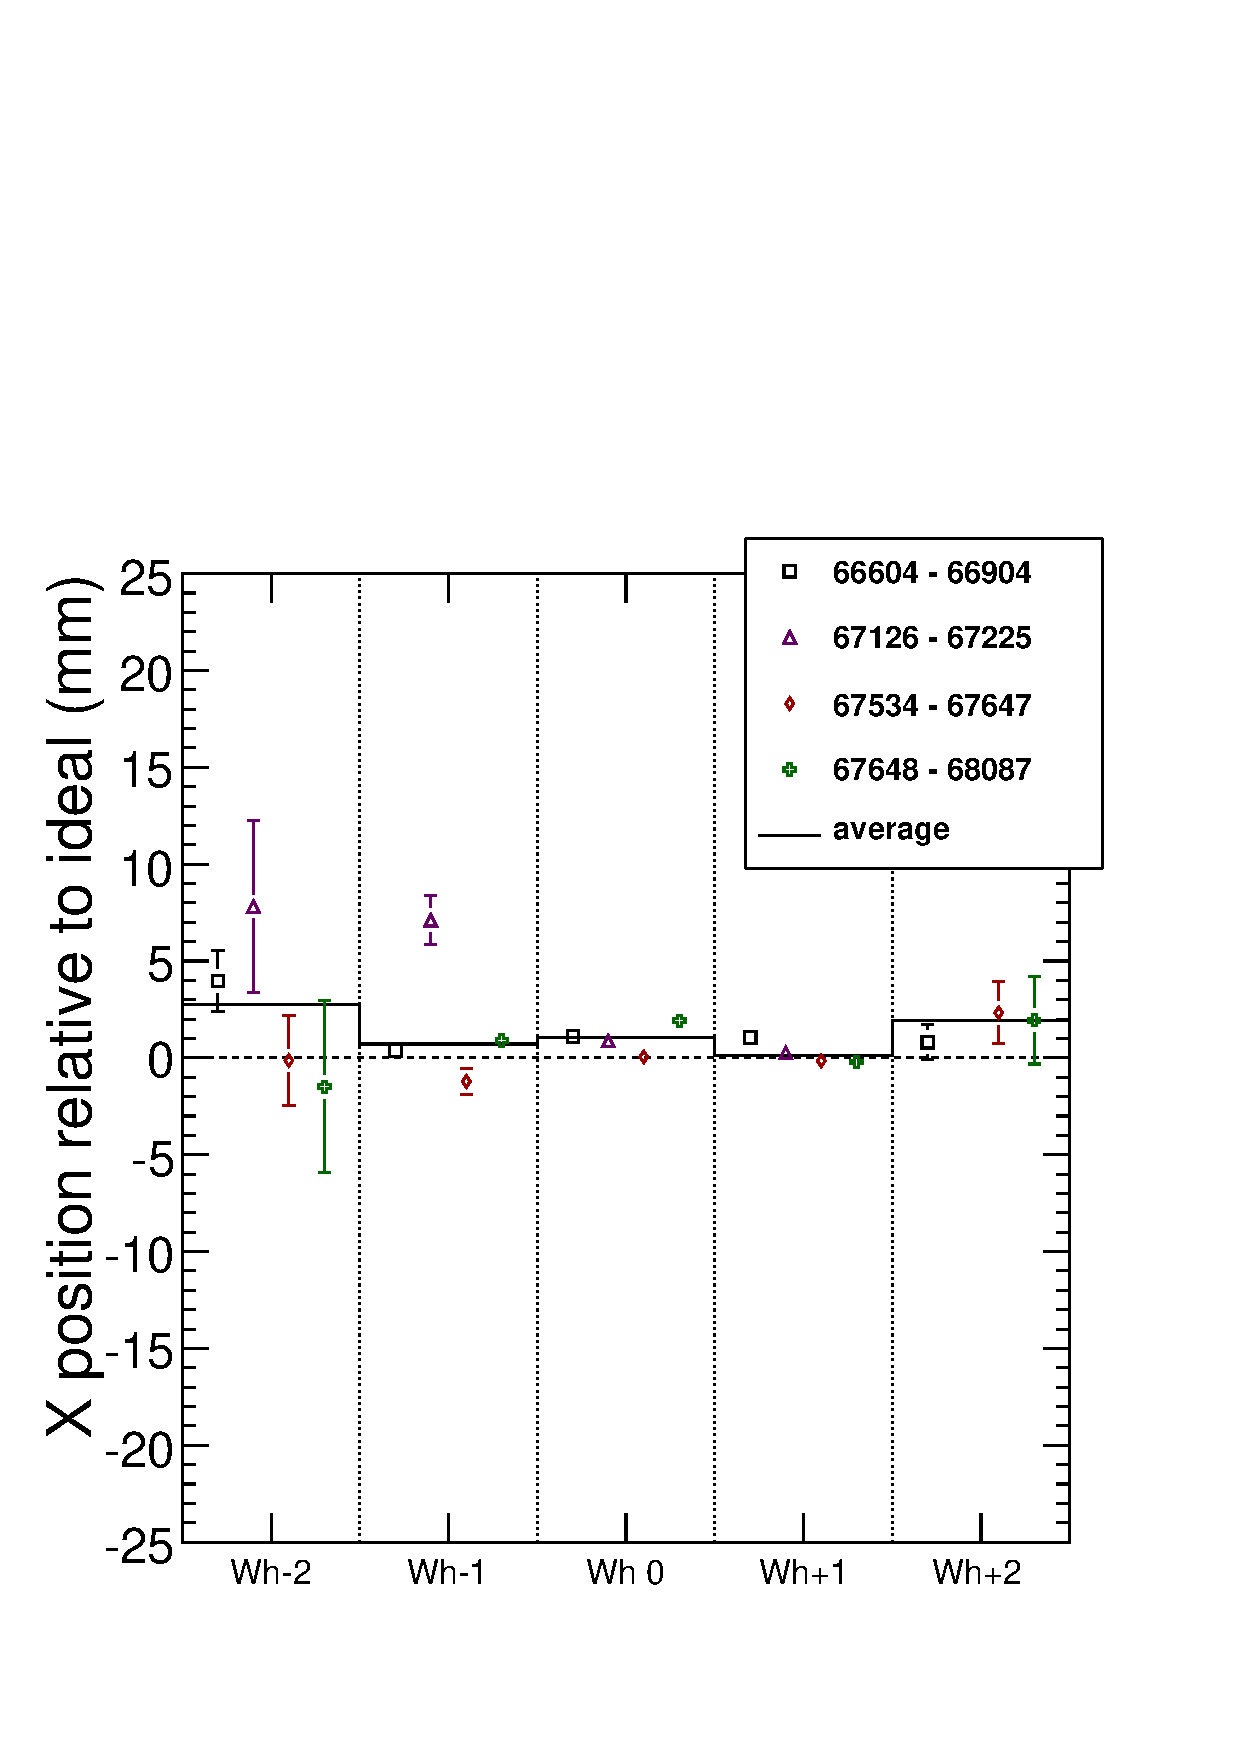
\includegraphics[width=\linewidth]{bydataset_MP_x.pdf}
\column{0.5\linewidth}
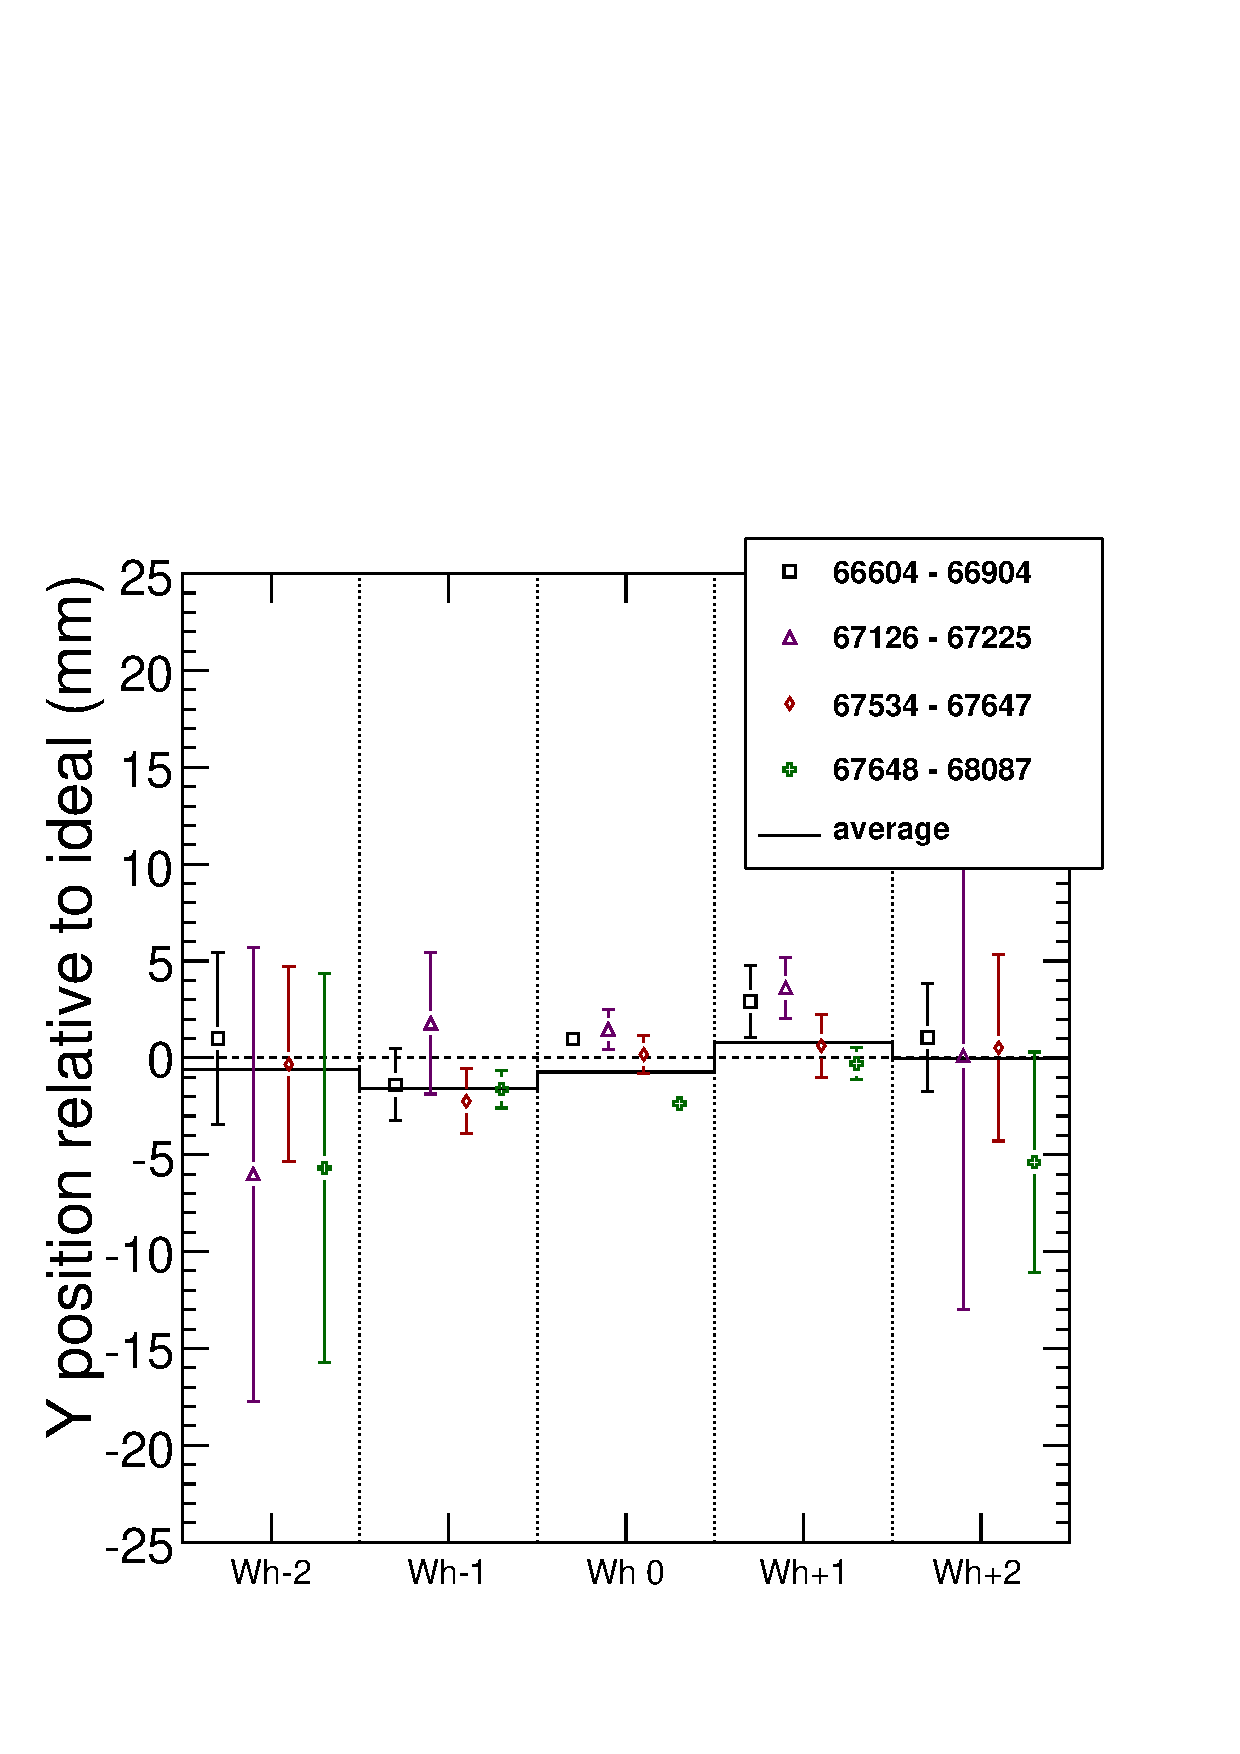
\includegraphics[width=\linewidth]{bydataset_MP_y.pdf}
\end{columns}}
\only<7>{\begin{columns}
\column{0.5\linewidth}
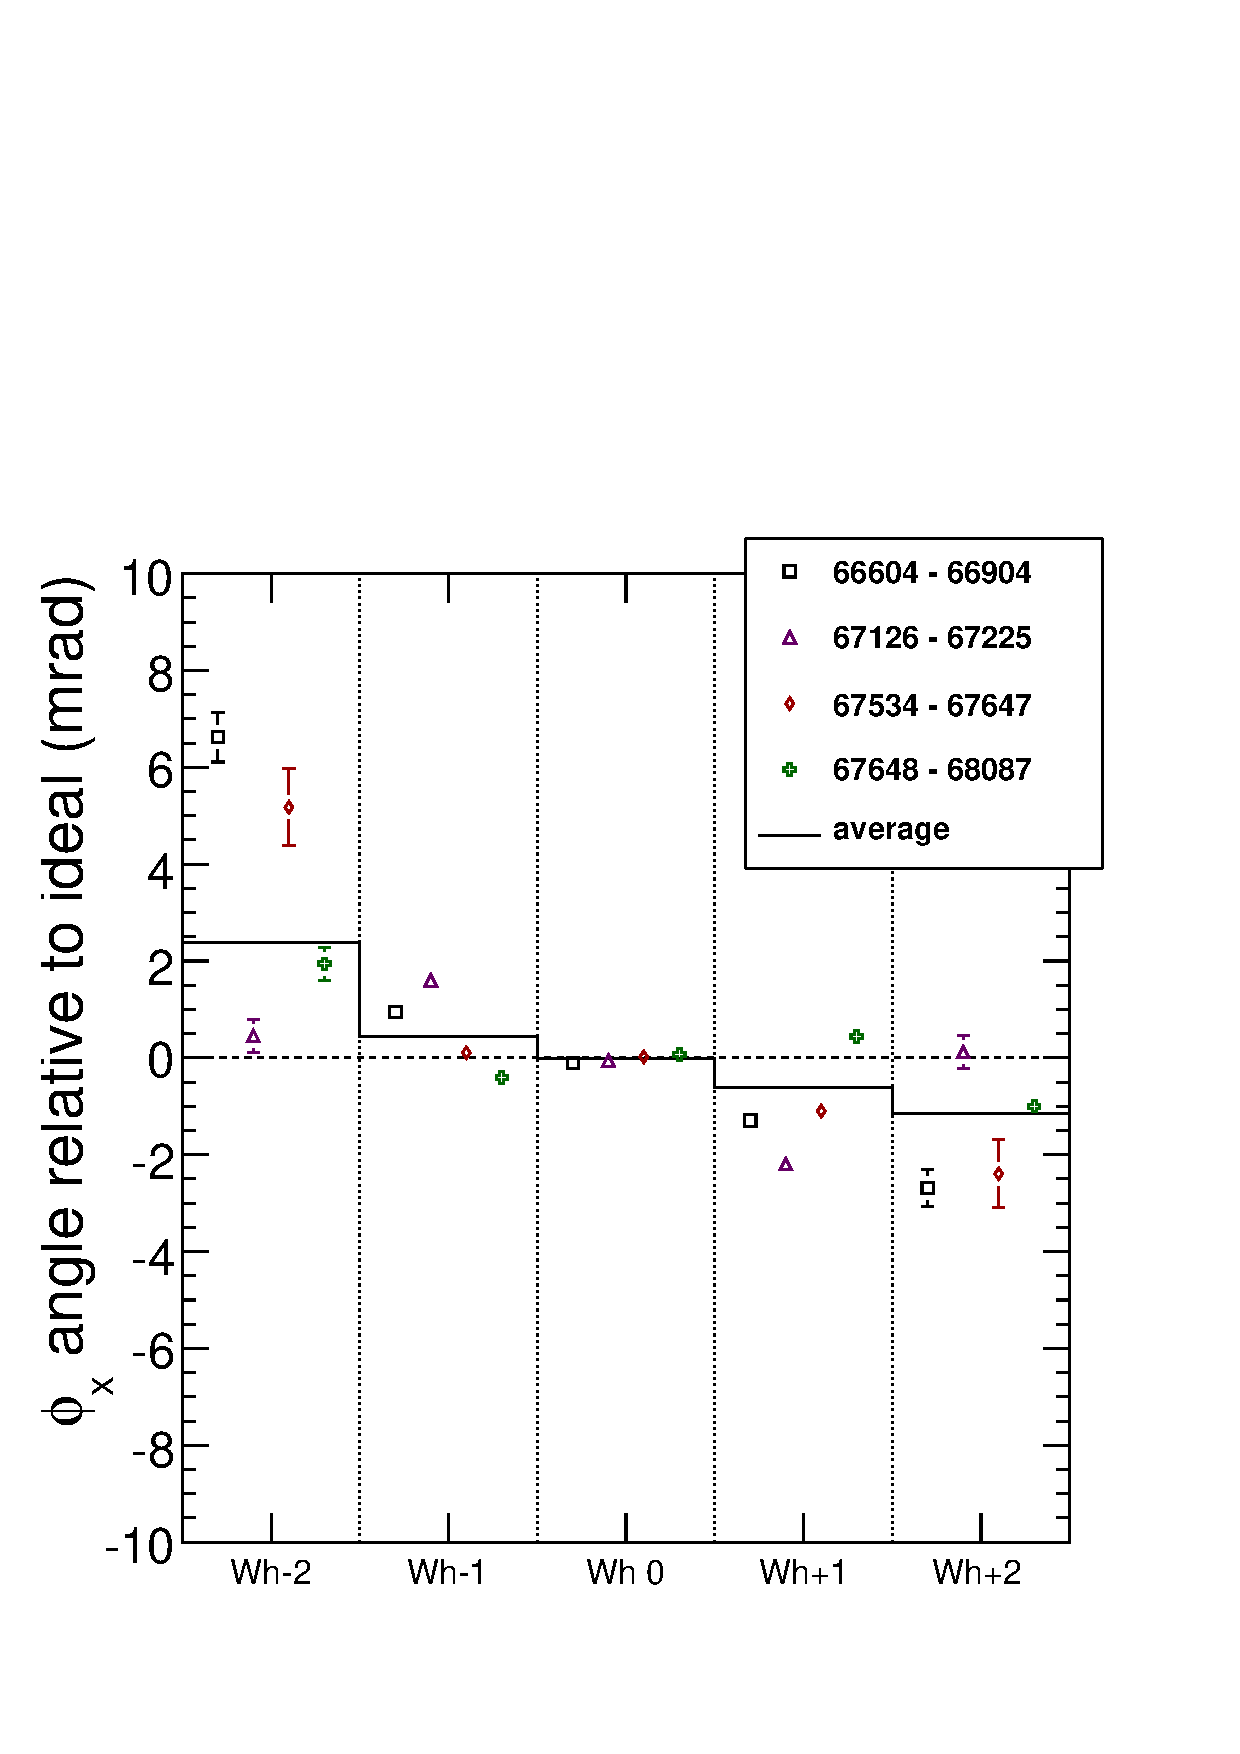
\includegraphics[width=\linewidth]{bydataset_HIPSC_phix.pdf}
\column{0.5\linewidth}
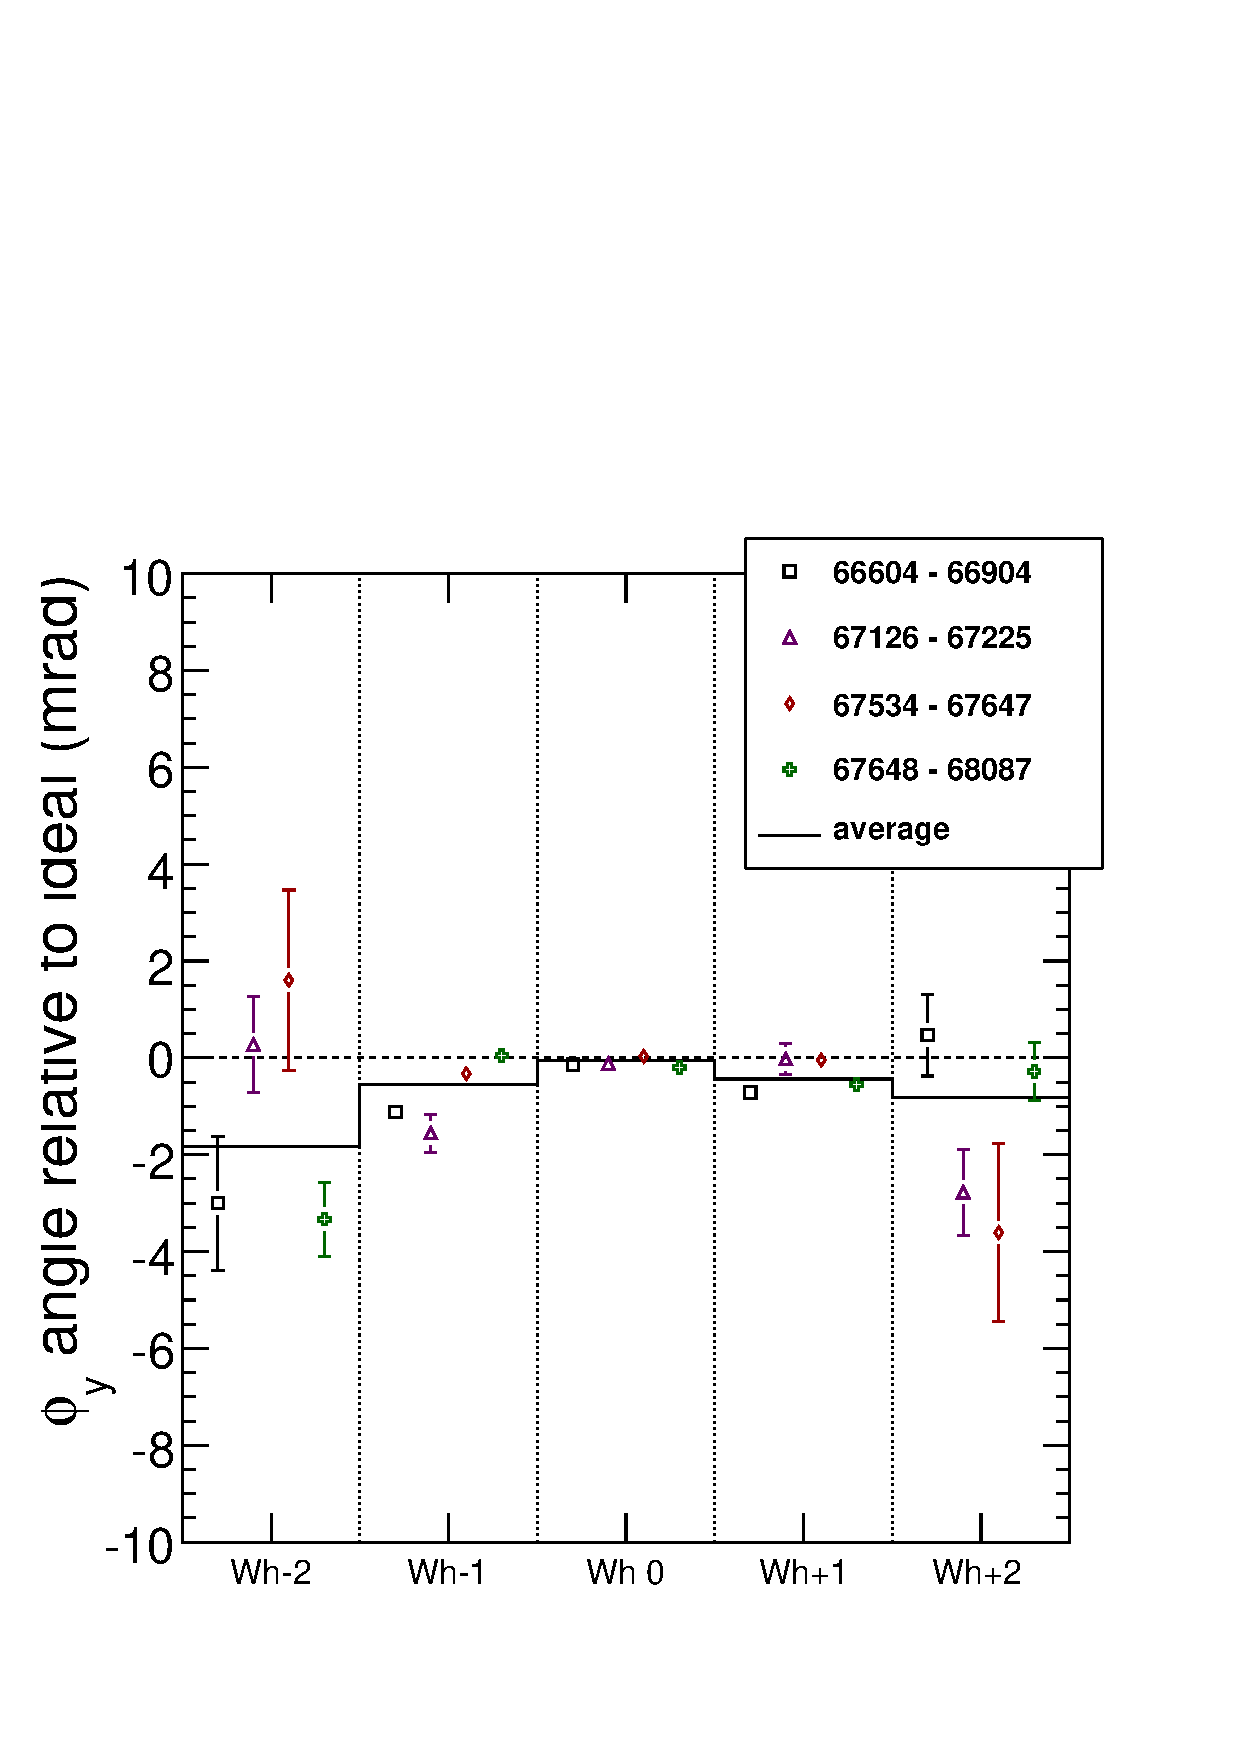
\includegraphics[width=\linewidth]{bydataset_HIPSC_phiy.pdf}
\end{columns}}
\only<8>{\begin{columns}
\column{0.5\linewidth}
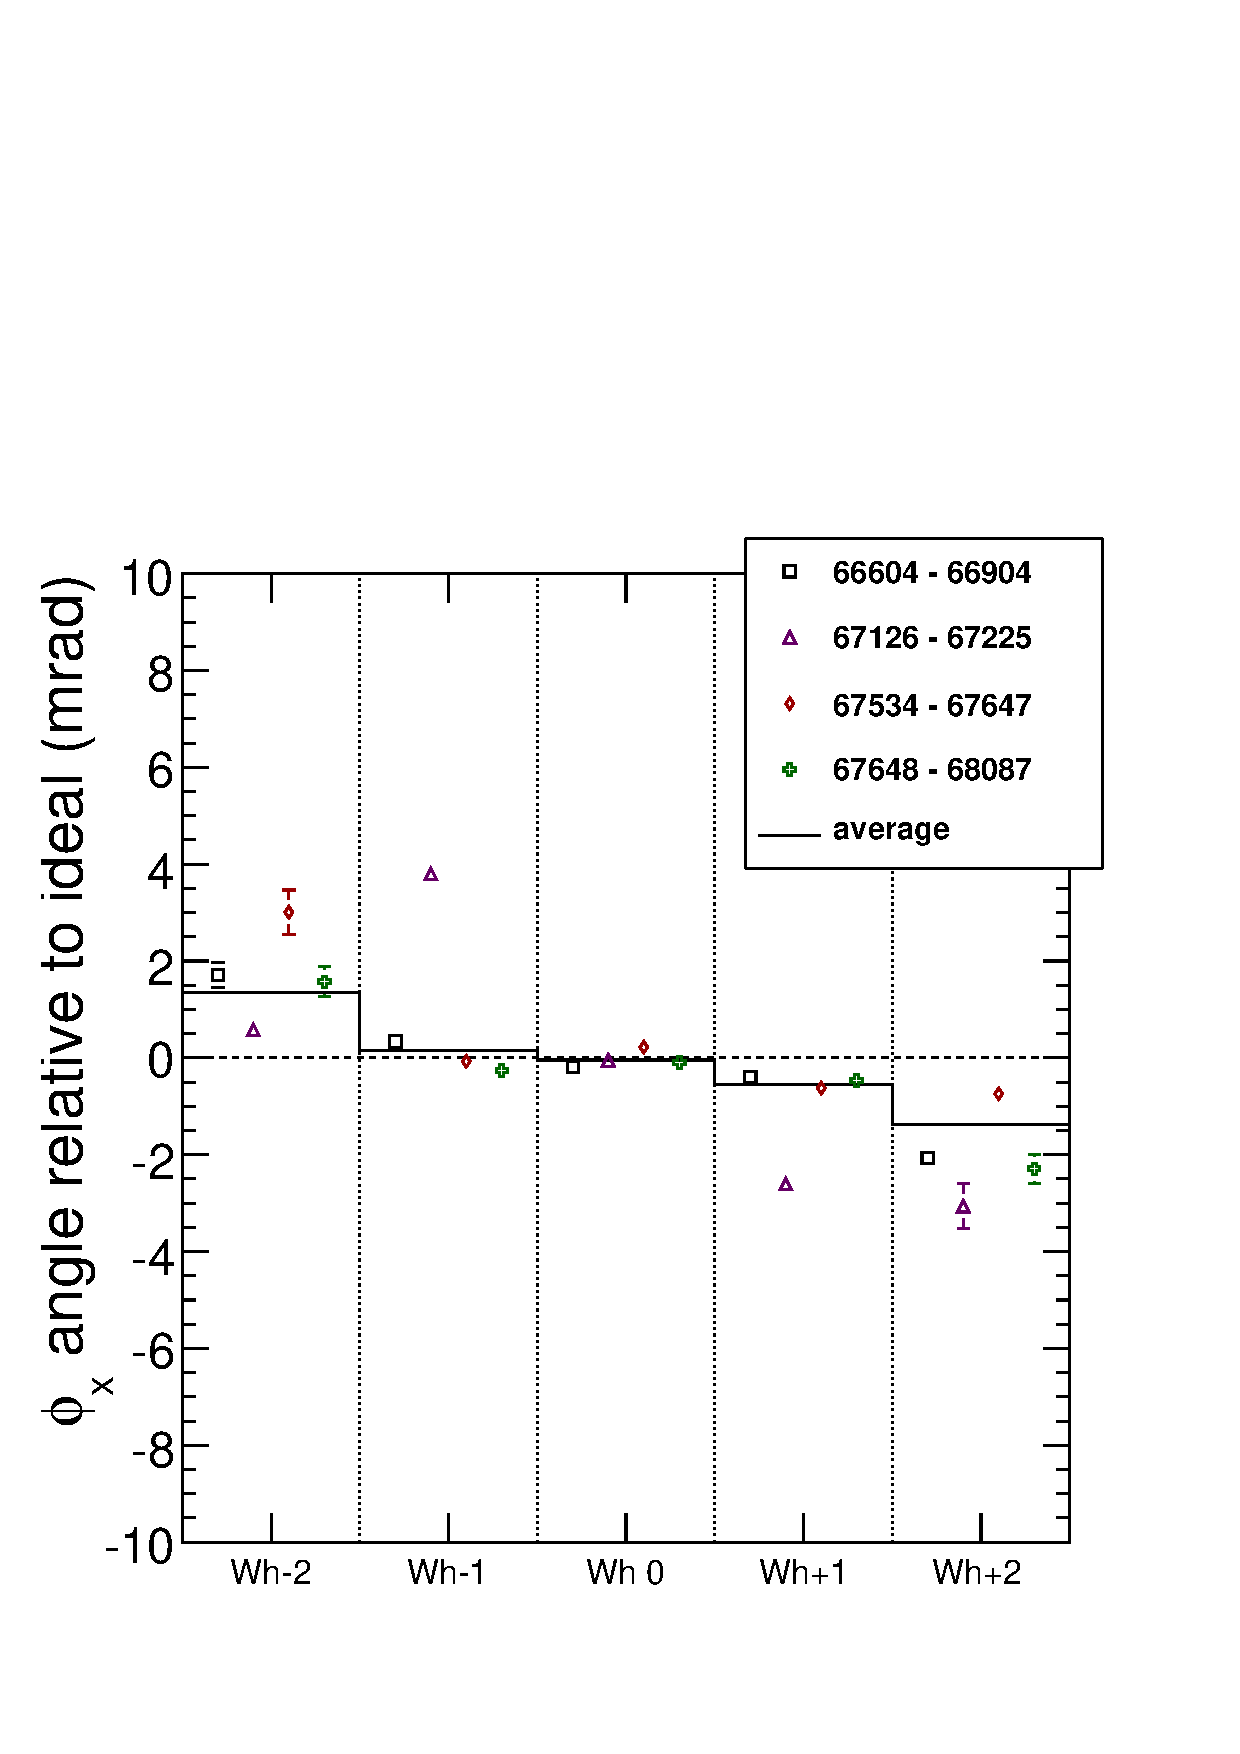
\includegraphics[width=\linewidth]{bydataset_MP_phix.pdf}
\column{0.5\linewidth}
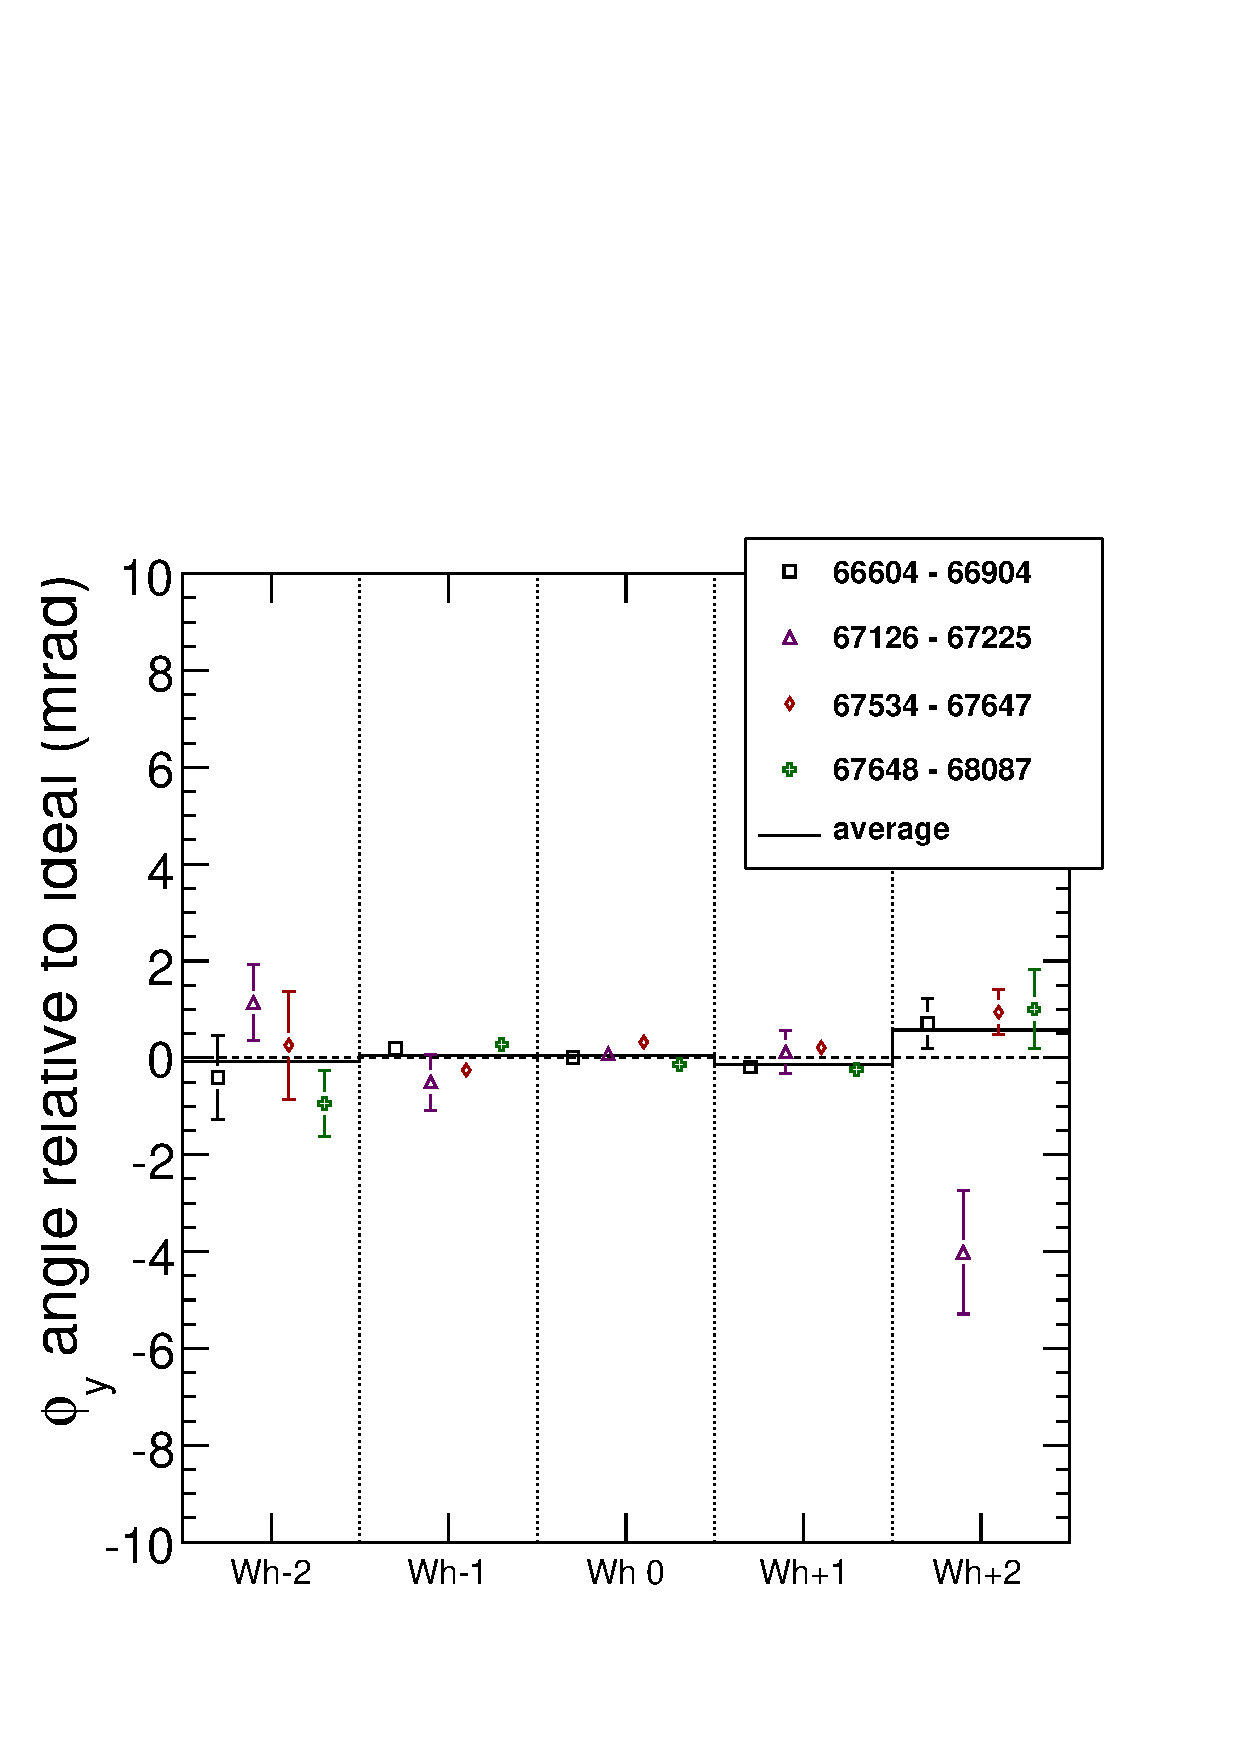
\includegraphics[width=\linewidth]{bydataset_MP_phiy.pdf}
\end{columns}}
\end{frame}

\begin{frame}
\frametitle{Conclusions}
\begin{itemize}\setlength{\itemsep}{0.25 cm}

\item Tracker MillePede alignment yields the most stable positions
  from one run range to the next

\item Uncertainties appear to be underestimated in barrel: switch to
  unweighted means (less precise, more robust)

\item Endcap will probably converge with $\left(\begin{array}{c c c} x &  & z \\ \phi_x & \phi_y & \phi_z \end{array}\right)$ floating

\item Should be compared to survey/hardware

\item Endcap results should be combined with hardware measurements of
  disk bowing, because inner rings are {\it extremely}
  statistics-limited in globalMuon cosmic rays

\item Alignment takes about 5 hours on about 100 CPUs (depending on
  dataset): we have time to prepare another, including the above
\begin{itemize}
\item Should four run ranges be combined?  I think so.
\end{itemize}

\end{itemize}
\label{numpages}
\end{frame}

\begin{frame}
\frametitle{Backup: tracker alignment study}

\vfill
\begin{itemize}
\item Largest run range (66604-66904)
\item Compare results using tracker alignment from CRUZET, CRAFT HIP with Survey Constraints, and CRAFT MillePede
\item Muon alignment is always MuonHIP, tracks only
\end{itemize}

\vfill
\vfill
\only<1>{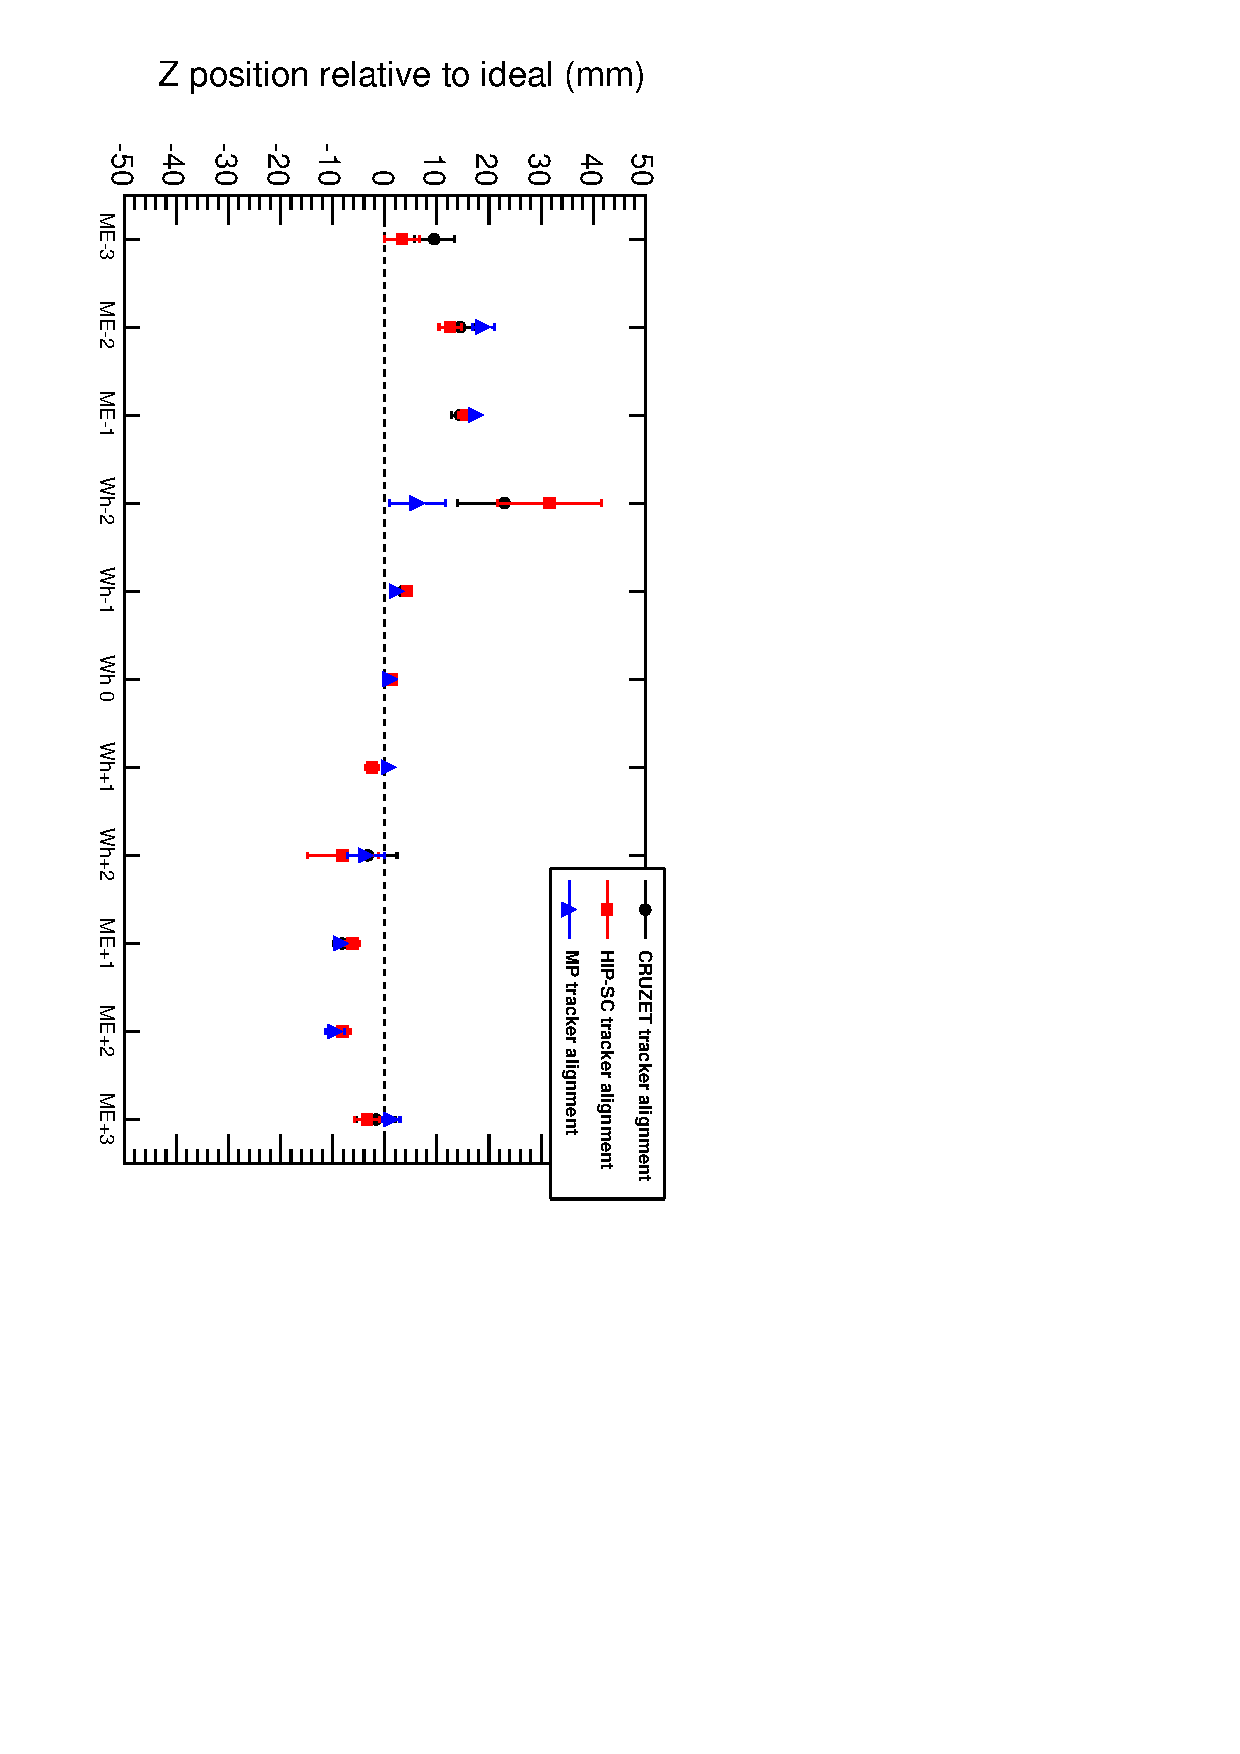
\includegraphics[height=\linewidth, angle=90]{compare_tracker_alignment_z.pdf}}
\only<2>{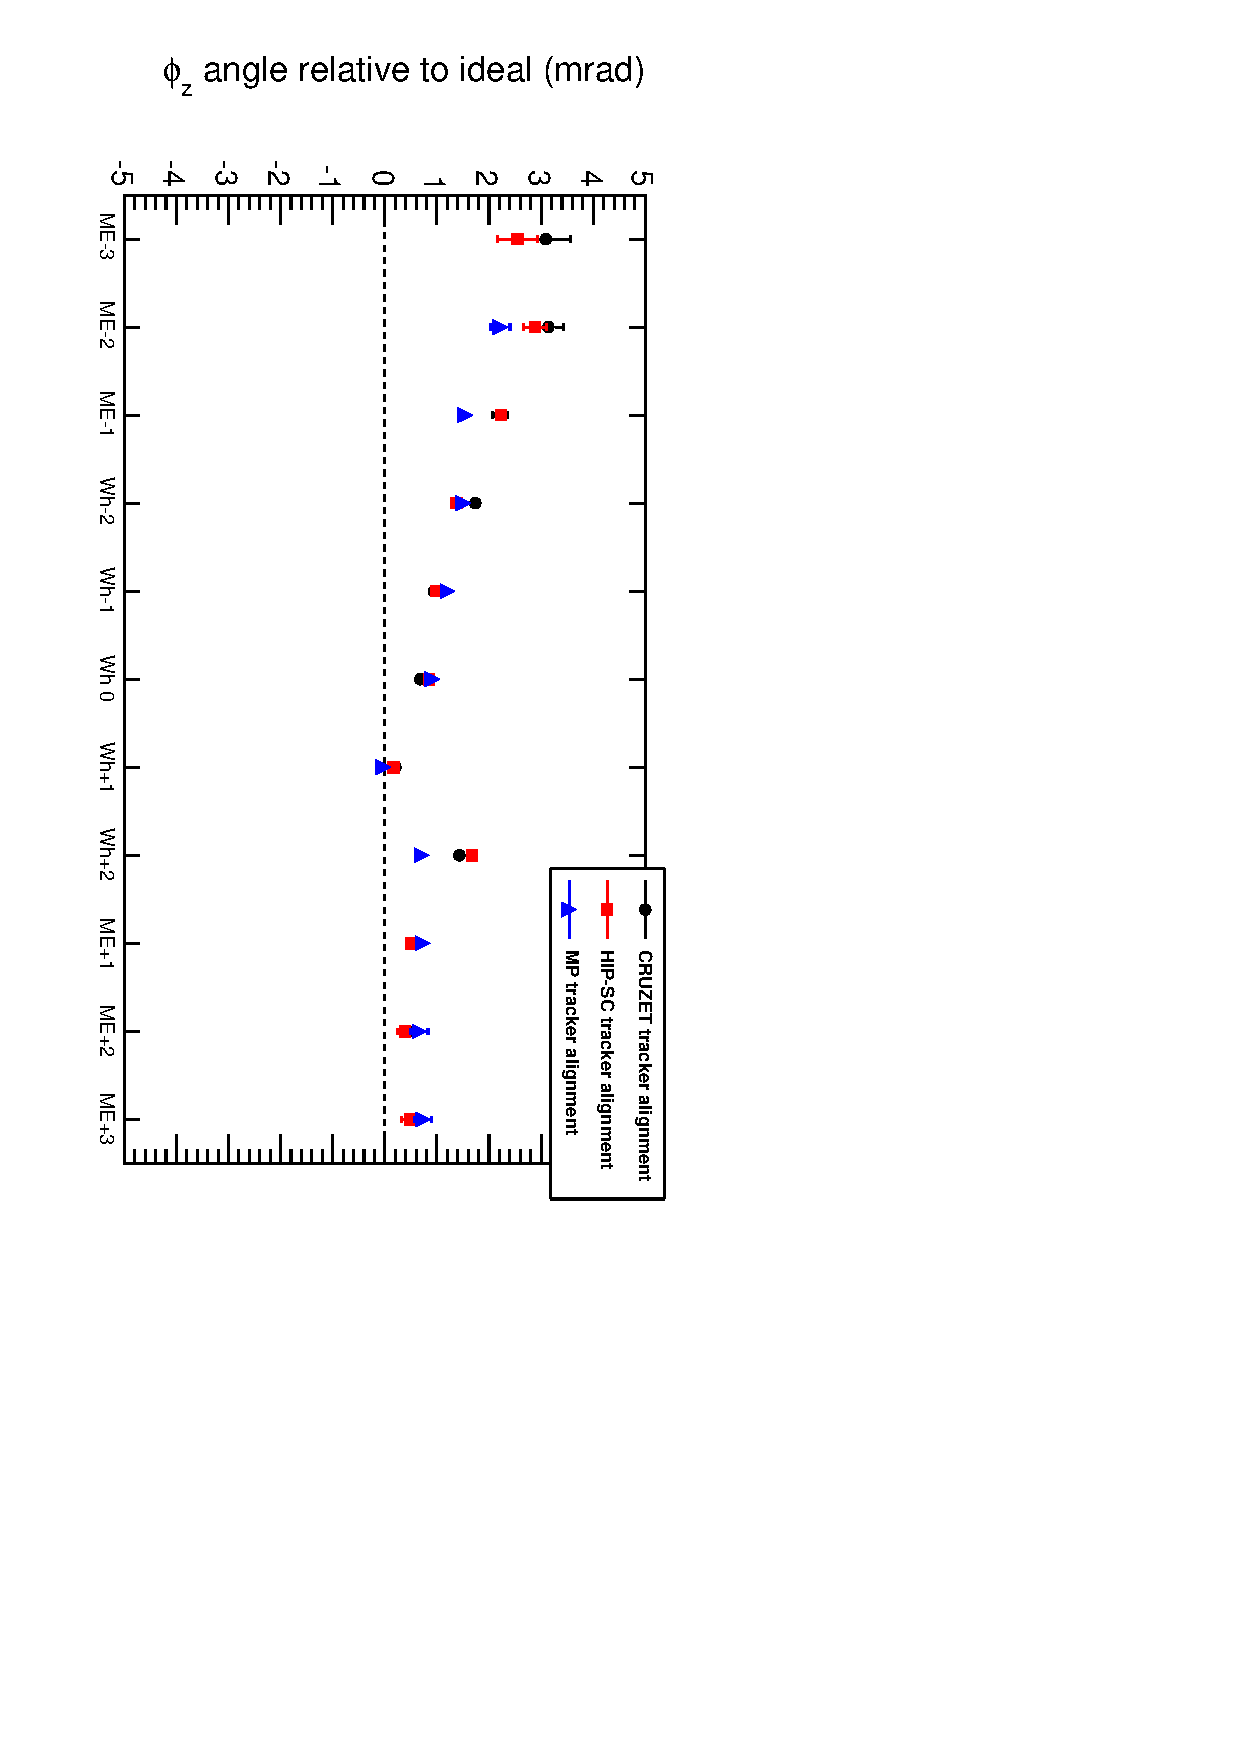
\includegraphics[height=\linewidth, angle=90]{compare_tracker_alignment_phiz.pdf}}
\only<3>{\begin{columns}
\column{0.5\linewidth}
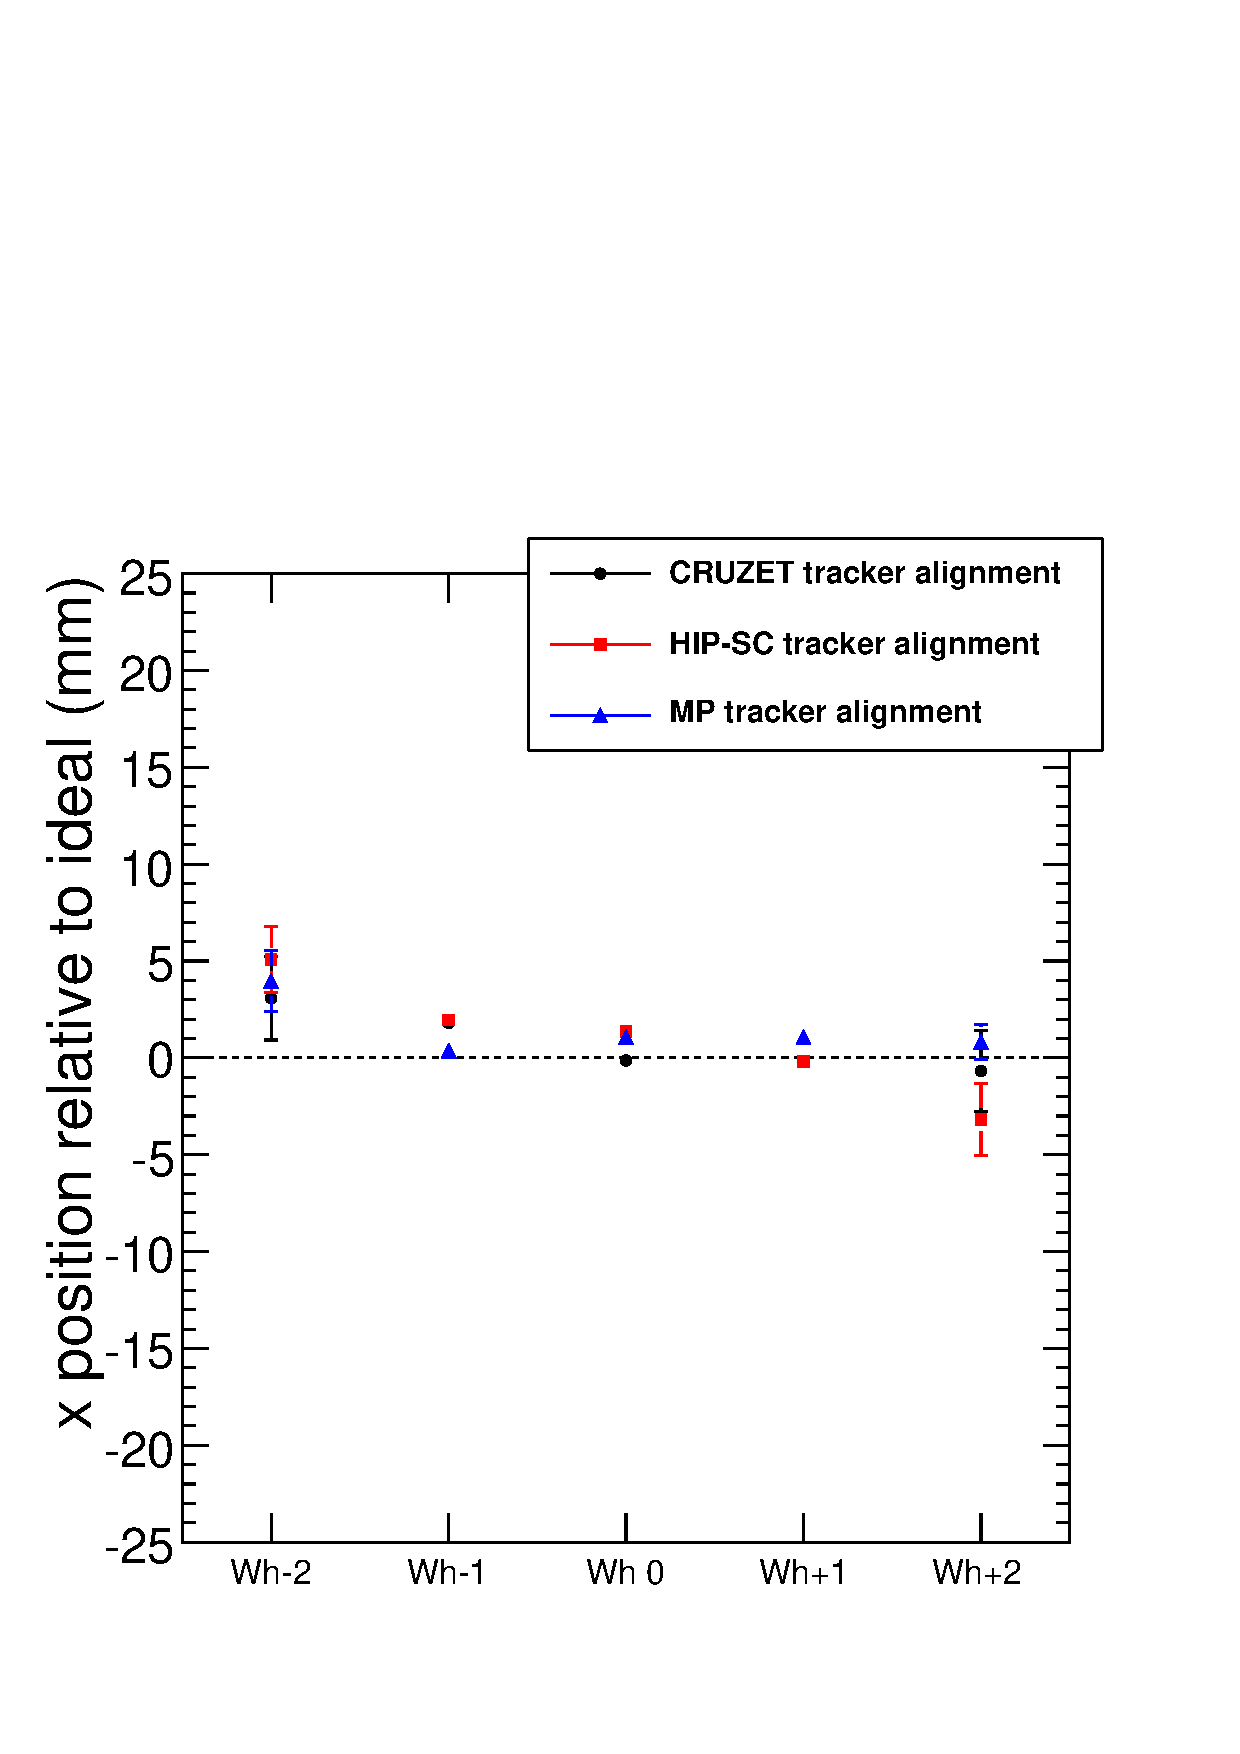
\includegraphics[width=\linewidth]{compare_tracker_alignment_x.pdf}
\column{0.5\linewidth}
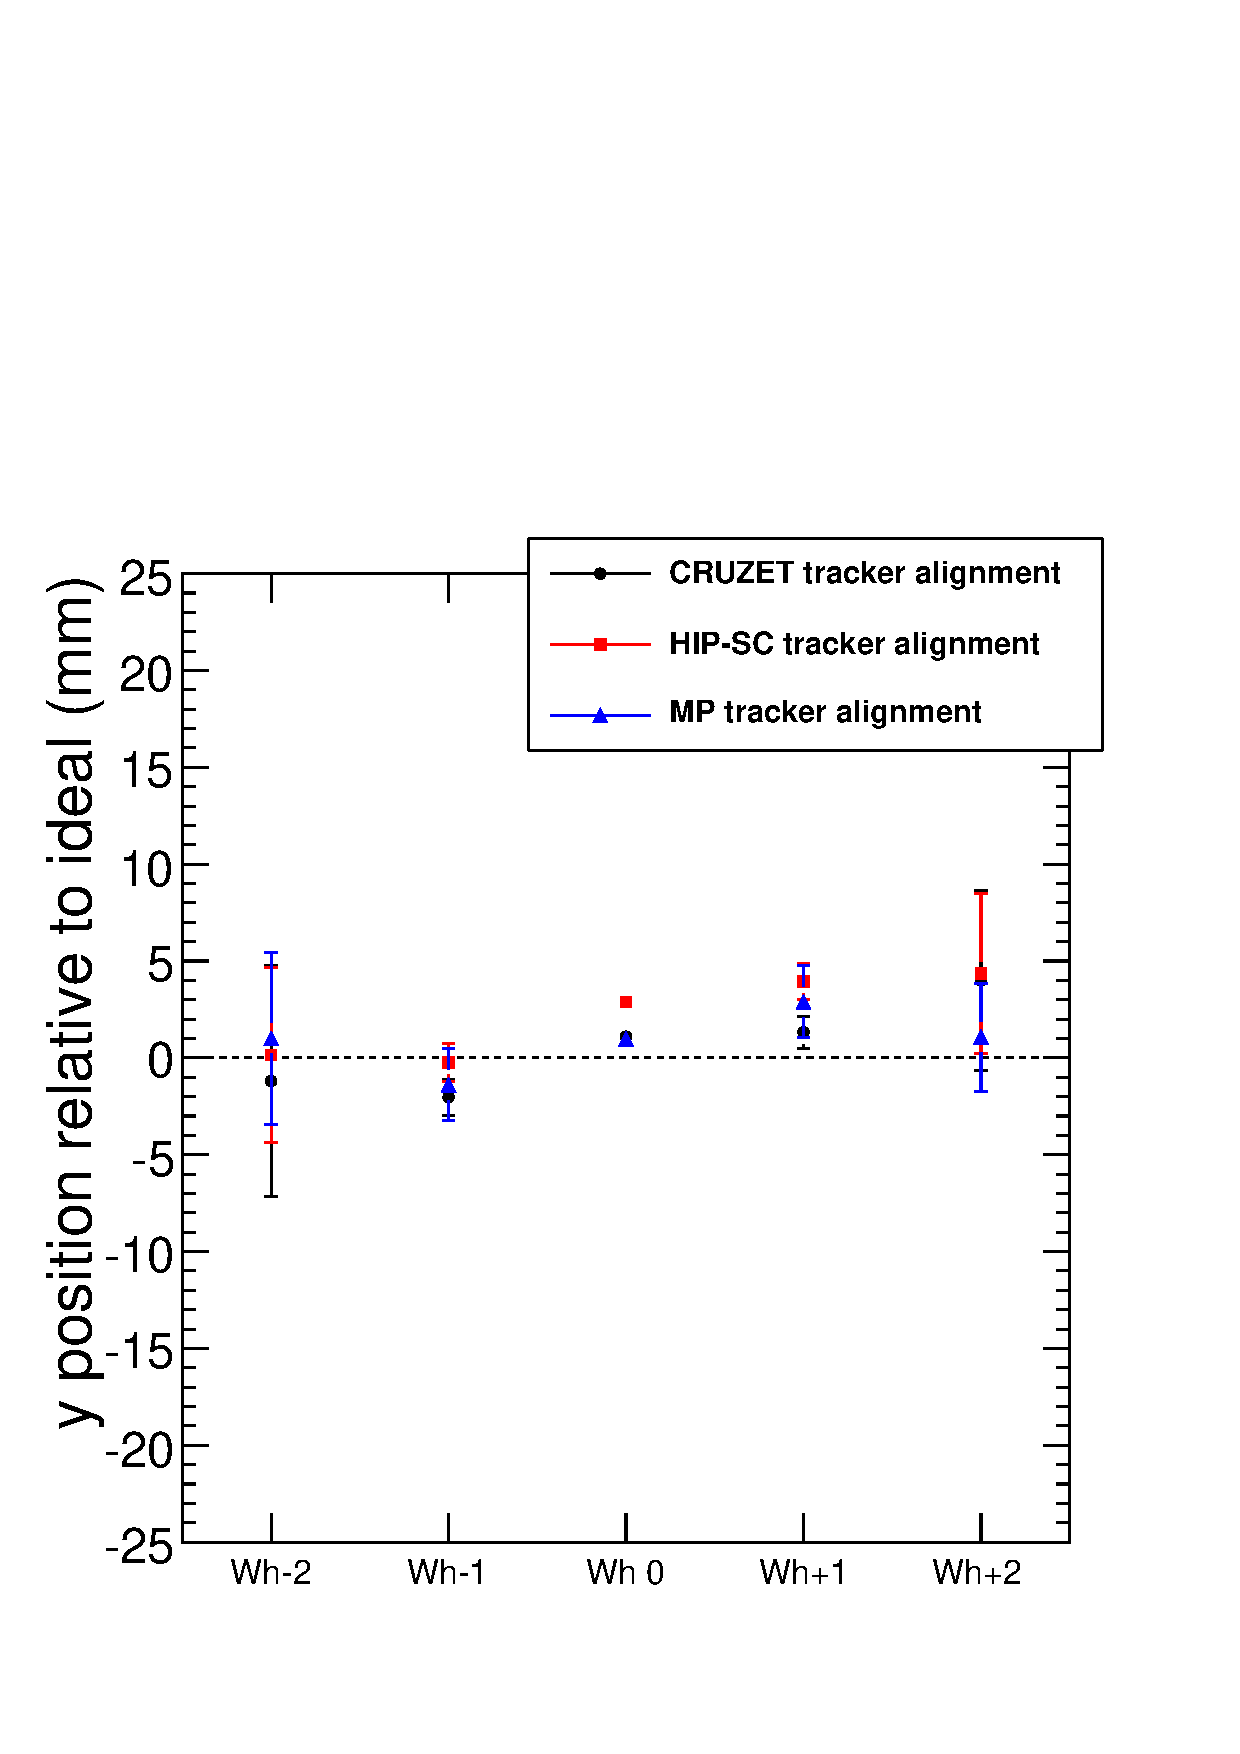
\includegraphics[width=\linewidth]{compare_tracker_alignment_y.pdf}
\end{columns}}
\only<4>{\begin{columns}
\column{0.5\linewidth}
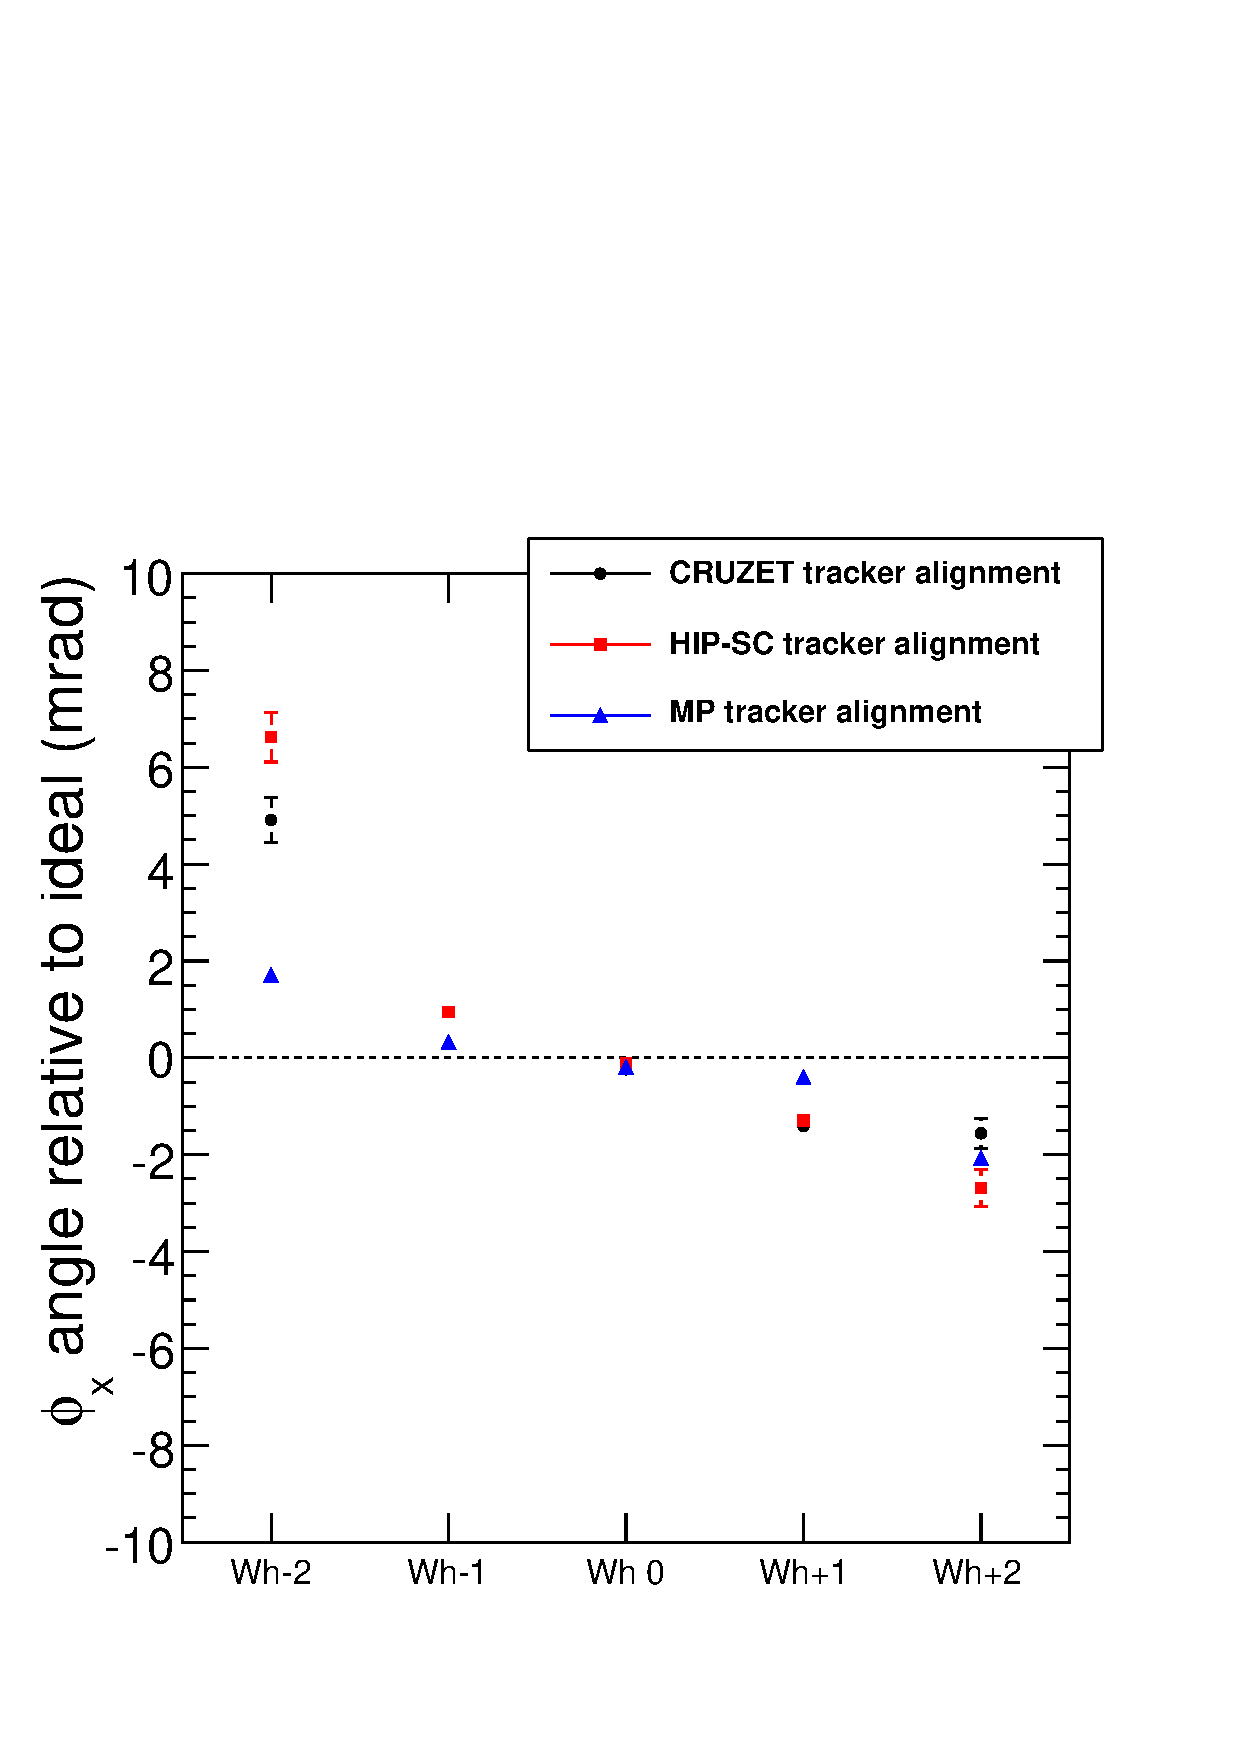
\includegraphics[width=\linewidth]{compare_tracker_alignment_phix.pdf}
\column{0.5\linewidth}
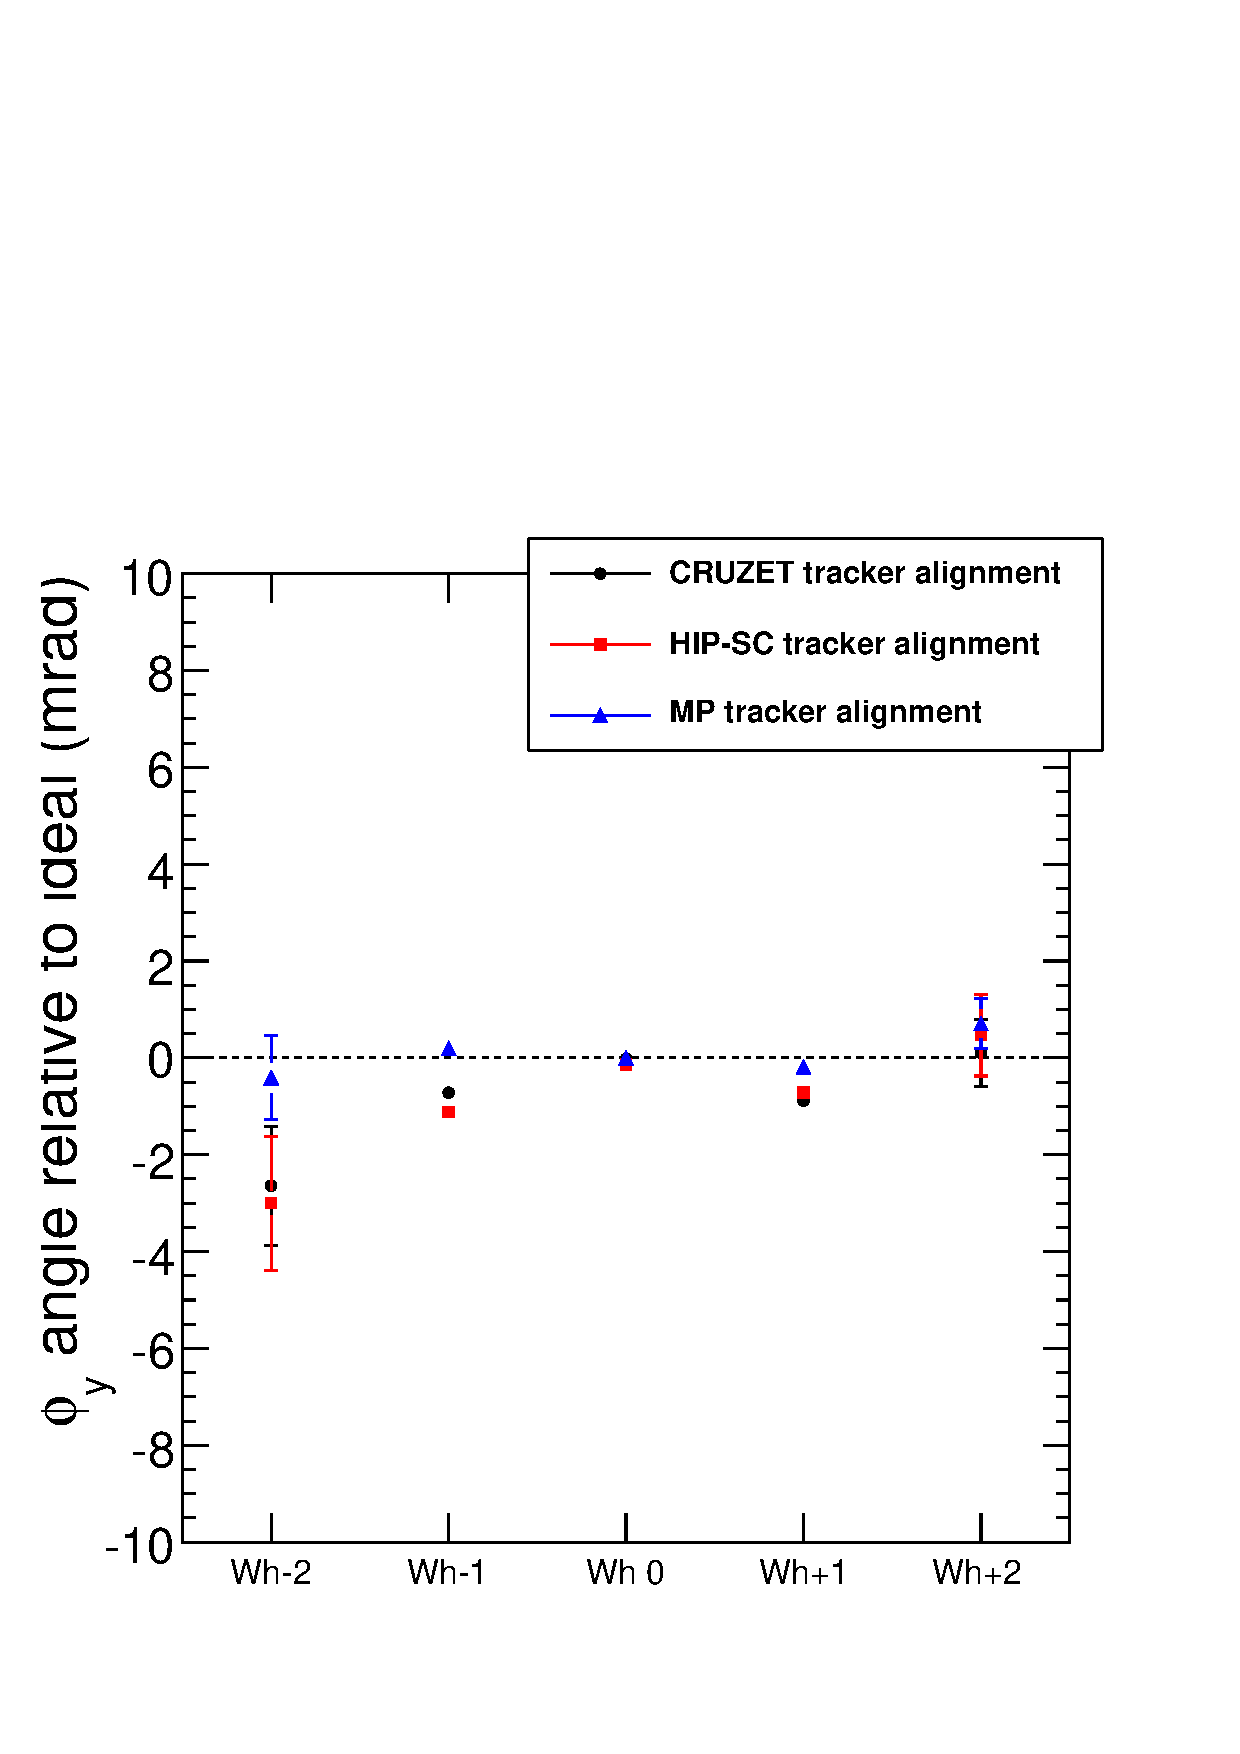
\includegraphics[width=\linewidth]{compare_tracker_alignment_phiy.pdf}
\end{columns}}
\end{frame}

\end{document}
